\documentclass{article}

% Language setting
% Replace `english' with e.g. `spanish' to change the document language
\usepackage[english]{babel}

% Set page size and margins
% Replace `letterpaper' with `a4paper' for UK/EU standard size
\usepackage[letterpaper,top=2.5cm,bottom=2.5cm,left=2cm,right=2cm,marginparwidth=1.75cm]{geometry}

% Useful packages
\usepackage{amsmath}
\usepackage{graphicx} % Required for including images
\usepackage{cite}     % Required for handling citations
\usepackage[colorlinks=true, allcolors=blue]{hyperref}

\usepackage{listings}
\usepackage{xcolor}
\RequirePackage{subfig} % current version of subfigures:
\usepackage{subcaption}
\usepackage{wrapfig}
\RequirePackage[utf8]{inputenc}
\RequirePackage[T1]{fontenc}
\RequirePackage{lmodern}
\RequirePackage{fancyhdr}
\usepackage{float}
\RequirePackage{numprint}				% styling of numbers


\usepackage{multirow}

% Define colors for syntax highlighting
\definecolor{keywordcolor}{RGB}{0,0,255}
\definecolor{commentcolor}{RGB}{0,128,0}
\definecolor{stringcolor}{RGB}{255,0,0}

% Set the style for C++ code
\lstdefinestyle{cppstyle}{
	language=C++,
	keywordstyle=\color{keywordcolor},
	commentstyle=\color{commentcolor},
	stringstyle=\color{stringcolor},
	basicstyle=\ttfamily,
	numbers=left,
	numberstyle=\tiny,
	stepnumber=1,
	numbersep=5pt,
	frame=single,
	tabsize=4,
	breaklines=true
}


% Define code style
\lstdefinestyle{cppstyle2}{
  language=C++,
  basicstyle=\scriptsize,
  keywordstyle=\color{blue}\ttfamily,
  stringstyle=\color{red}\ttfamily,
  commentstyle=\color{orange}\ttfamily,  
%  basicstyle=\ttfamily\footnotesize,
%  keywordstyle=\color{blue},
%  commentstyle=\color{green!50!black},
%  stringstyle=\color{red},
  numbers=left,
  numberstyle=\tiny, 
  stepnumber=1,
  breaklines=true,
  backgroundcolor=\color{gray!10},
  frame=single
}


\titlepageAbschluss	{<<TITLE OF THESIS>>}% title
{<<MY NAME>>}% Author
{<<THE DATE>>}% date
{<<MATRICULATION NUMBER>>}%  matr. nr.
{Prof. Dr.-Ing. Dr. h.c. Hubert Roth}% 1st examiner
{M.Sc. <<SUPERVISOR>>}% 2nd examiner
{Bachelorarbeit/Studienarbeit/Masterarbeit}% doc type


\title{Self Balancing Robot}
\author{Muhammad Haris Mujeeb}

\begin{document}

\maketitle

\begin{abstract}
This report details the design and implementation of a two-wheeled self-balancing robot, a system that embodies the classic inverted pendulum challenge. The robot employs an MPU6050 inertial measurement unit (IMU) for precise state estimation, with sensor data fusion accomplished using a Kalman filter. A Proportional-Integral-Derivative (PID) control algorithm is implemented to ensure robust balance and stability. The system is designed to support remote monitoring and control, broadening its applicability across diverse scenarios. The firmware for the Arduino Nano was developed using \href{https://platformio.org/}{PlatformIO}, and the full project, including source code and comprehensive documentation, is accessible in this \href{https://github.com/haris-mujeeb/Self-Balancing-Robot}{GitHub repository}.
\end{abstract}

\thispagestyle{empty}
\tableofcontents
\listoffigures
\listoftables
\newpage


\section{Introduction}
\subsection{Background \& Motivation}
Two-wheeled vehicles are generally more agile, allowing easier navigation through tight spaces, making them ideal for congested environments. Their lighter weight and compact size facilitate easier handling while also enhancing energy efficiency. In addition, they are typically less expensive to purchase and maintain, increasing accessibility for a wider range of users.
A good base model to build such robot is \href{https://www.elegoo.com/products/elegoo-tumbller-self-balancing-robot-car}{ELEGOO Tumbler} (shown in Fig. 
\ref{fig:tumbler}), which provided nearly all the hardware required as a DIY kit.

\begin{figure}[h]
	\centering
	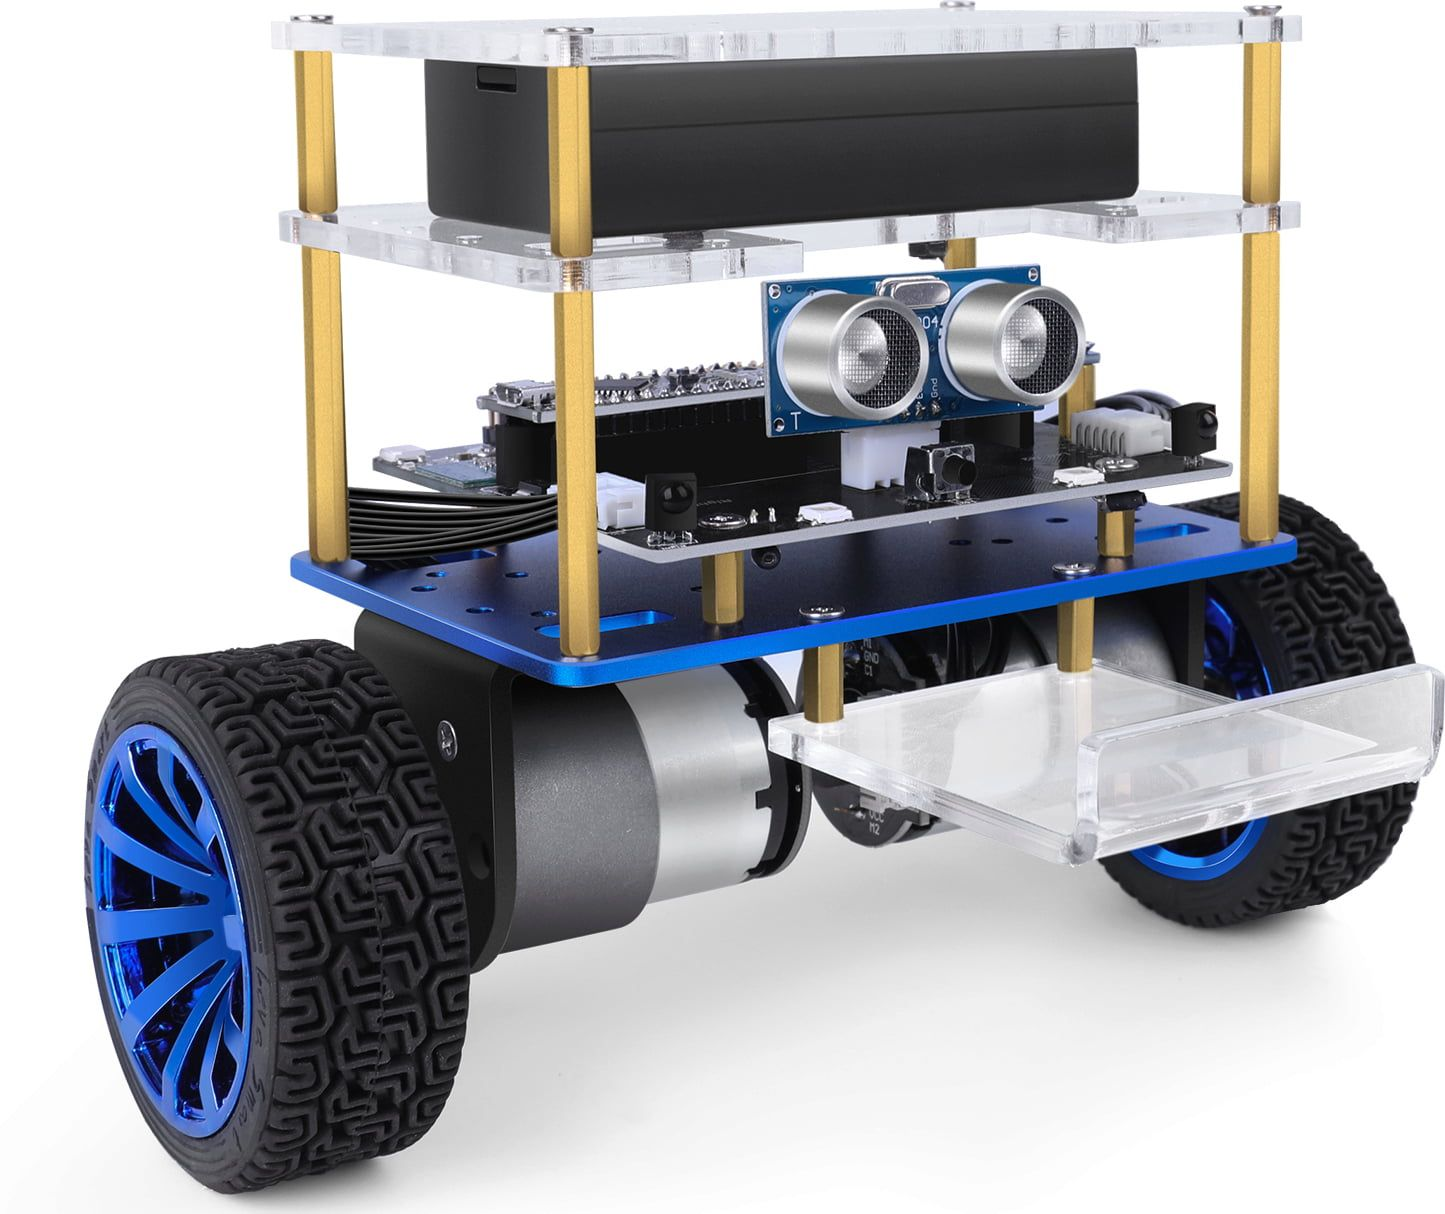
\includegraphics[height=6cm]{assets/tumbller.jpg}
	\caption{\label{fig:tumbler} ELEGOO Tumbler which was used for this project \cite{tumbller}.}
\end{figure}

\subsection{Project Objectives}
The primary objectives of this project are as follows:
\begin{itemize}
	\item To design and implement a two-wheeled self-balancing robot capable of maintaining stability using sensor feedback and control algorithms.
	\item To develop a cascaded PID control system for real-time balance and motion control, ensuring robustness and responsiveness.
	\item To integrate an MPU6050 inertial measurement unit (IMU) for accurate state estimation, utilizing sensor fusion techniques such as a Kalman filter.
	\item To enable remote monitoring and control of the robot, enhancing its versatility for various applications.
	\item To document the design, implementation, and tuning processes, providing a comprehensive resource for future development and replication.
\end{itemize}


\section{Literature Review}
Two-wheeled self-balancing robots have been widely studied as a variant of the classic inverted pendulum problem, requiring advanced control strategies to maintain stability. Various approaches, including Proportional-Integral-Derivative (PID) control \cite{matlab_inverted_pendulum}, Linear Quadratic Regulator (LQR)~\cite{10193276} have been explored to achieve robust balancing and motion control.

Xu and Duan~\cite{1174486} demonstrated that the Linear Quadratic Regulator (LQR) controller outperforms the pole-placement controller in both simulation and real-time control scenarios.

Kalman filtering has been extensively used for sensor fusion in such systems, particularly for integrating accelerometer and gyroscope data to obtain accurate state estimates. Studies have demonstrated that complementary and extended Kalman filters significantly improve stability and noise rejection in sensor-driven control systems.

Recent advancements in autonomous navigation for self-balancing robots have incorporated Simultaneous Localization and Mapping (SLAM) techniques, LiDAR-based obstacle detection, and machine learning-based adaptive control methods \cite{Tsai_Chih_2008} \cite{Ranasinghe_Vidanapathirana_2019}. These improvements enable real-time path planning and environmental interaction, making self-balancing robots more suitable for real-world applications such as personal mobility, surveillance, and industrial automation.

This project builds upon these existing methodologies by implementing a Kalman filter for sensor fusion and employing PID-based control to achieve stable balancing and maneuverability. Future work aims to integrate more advanced control and navigation techniques for enhanced autonomy and performance.

\subsection{Scope of Work}
The scope of this project encompasses the following key areas:
\begin{itemize}
	\item \textbf{Hardware Integration:} Assembling and configuring the ELEGOO Tumbler platform, including the MPU6050 IMU, motor drivers, and encoders.
	\item \textbf{Software Development:} Implementing firmware for the Arduino Nano microcontroller using PlatformIO, focusing on sensor data acquisition, control algorithms, and communication protocols.
	\item \textbf{Control System Design:} Designing and tuning a cascaded PID control loop for pitch, yaw, and position control, ensuring stable and precise operation.
	\item \textbf{Sensor Fusion:} Utilizing a Kalman filter to fuse data from the IMU, improving the accuracy of state estimation and control.
	\item \textbf{Testing and Validation:} Conducting extensive testing to evaluate the robot's performance under various conditions, followed by iterative refinement of the control parameters.
	\item \textbf{Documentation and Open-Source Contribution:} Providing detailed documentation, including schematics, code, and tuning guidelines, and making the project available on a \href{https://github.com/haris-mujeeb/Self-Balancing-Robot}{GitHub repository} for open-source collaboration \cite{opensource}.
\end{itemize}

\begin{figure}[h]
	\centering
	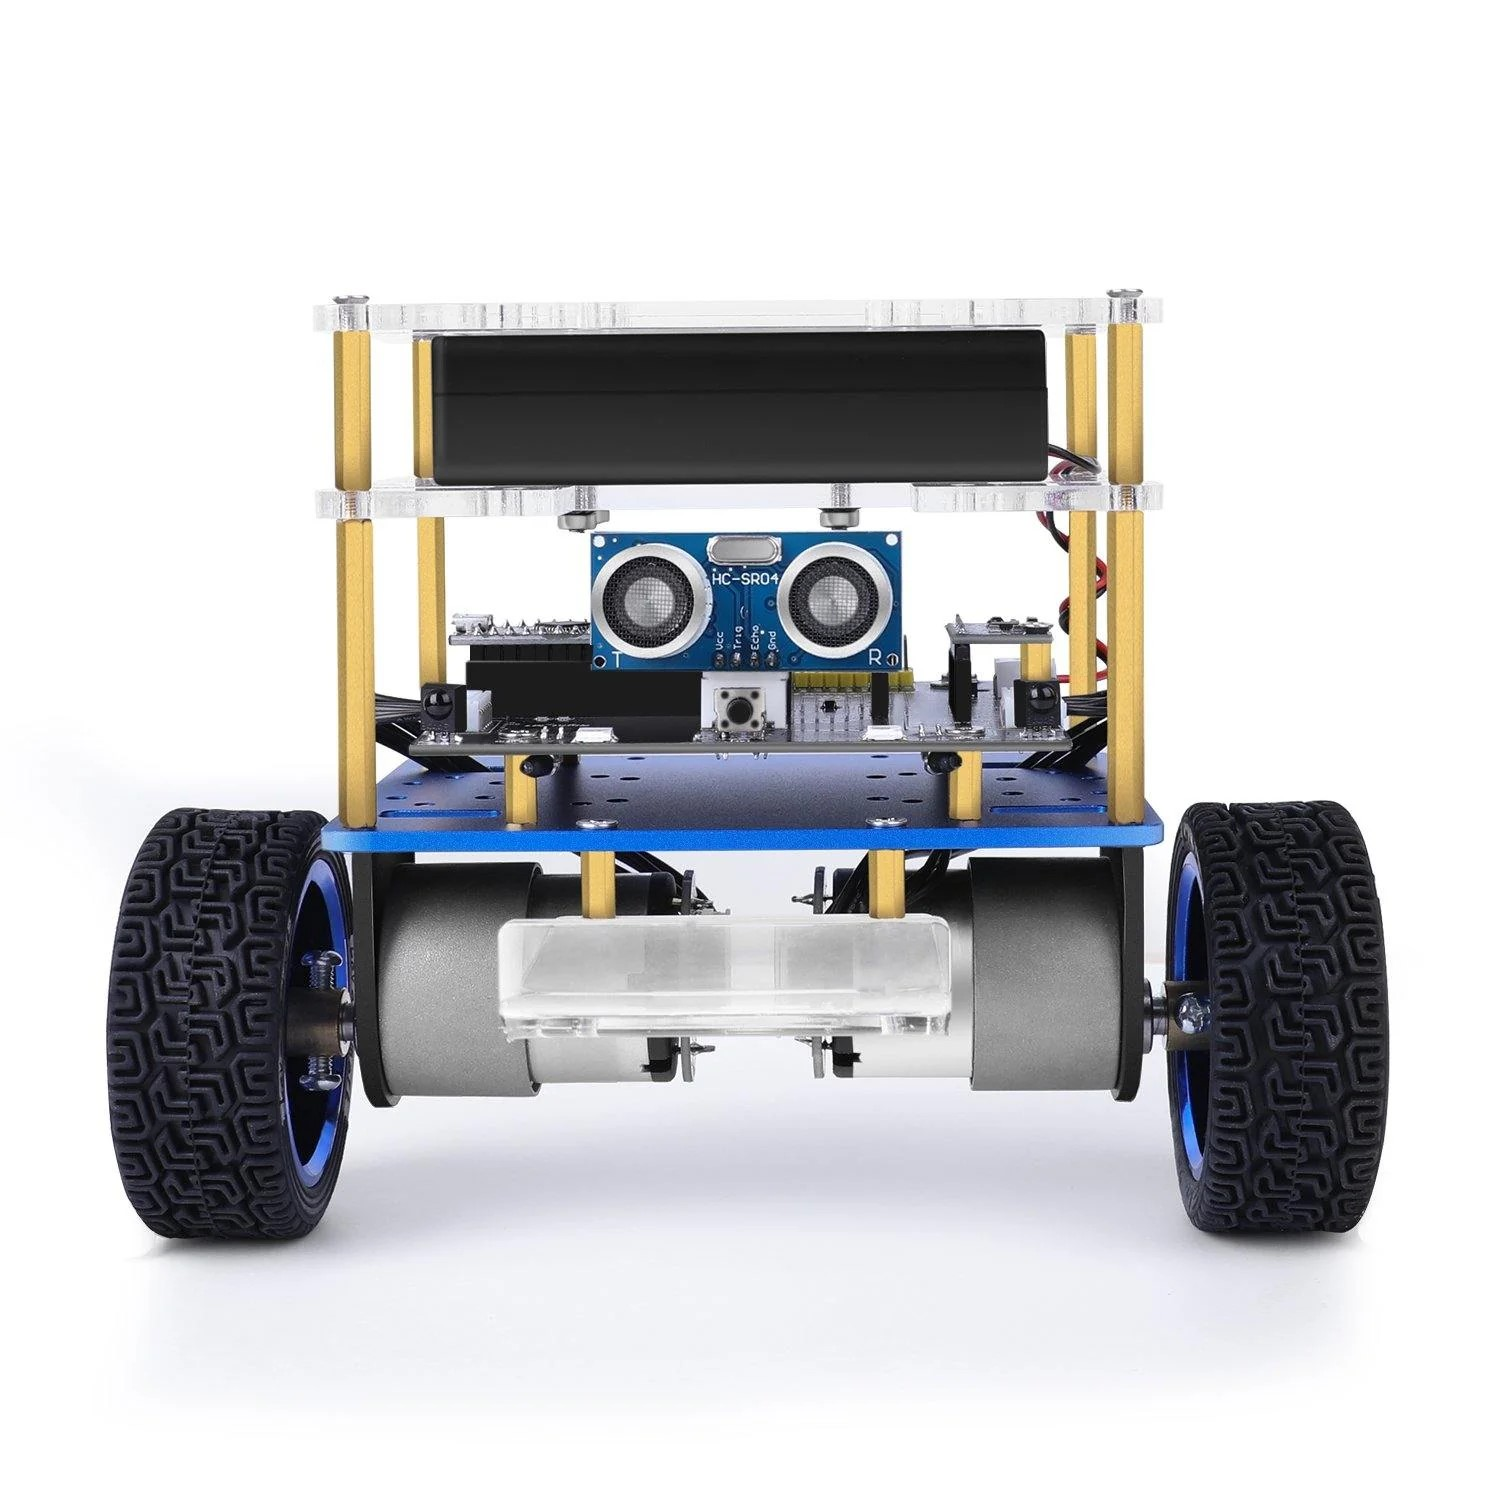
\includegraphics[height=6cm]{assets/tumbller2.jpg}
	\caption{\label{fig:tumbler2} ELEGOO Tumbler \cite{tumbller}.}
\end{figure}
\subsection{Mathematical Modelling}
The physical problem of the balancing robot is well described by the widely analyzed inverted pendulum model. This system is typically represented as a rigid rod attached to a joint, mounted on a rigid cart that moves in a single direction.

\begin{figure}[H]
	\centering
	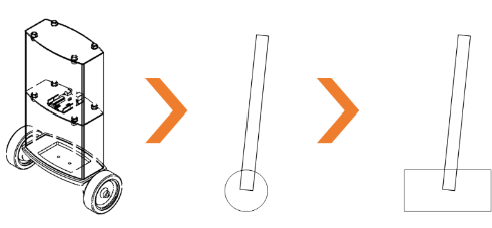
\includegraphics[width=0.6\textwidth]{assets/simplified-inverted-pendulem.png}
	\caption{Simplified inverted pendulum model for the balancing robot \cite{10193276}.}
	\label{fig:pendulum_model}
\end{figure}


For simplification, the wheelbase of the robot is assumed to behave like a cart sliding on a frictionless surface. This modeling approach follows Prasad and Tyagi \cite{prasad_optimal_2014}, and the MathWorks tutorial on the inverted pendulum \cite{matlab_inverted_pendulum}. 

To ease mathematical formulation, the pendulum’s motion is restricted to one degree of freedom, with the angle $\theta$ evolving in the xy-plane, see Figure~\ref{fig:pendulum_model}.

\begin{figure}[H]
	\centering
	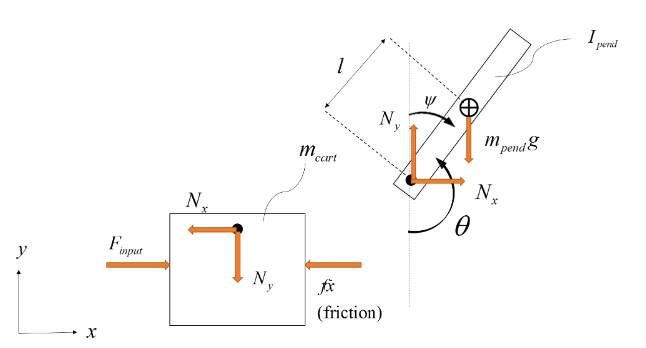
\includegraphics[width=0.6\textwidth]{assets/FBD-inverted-pendulum.png}
	\caption{Free-body diagram for inverted pendulum\cite{10193276}.}
	\label{fig:FBD-inverted-pendulum}
\end{figure}


\subsubsection{State Equations}
The state equations for the system, describing the evolution of the state variables over time, are given by
\begin{equation}
	F_{input} = (m_{cart} + m_{pend}) \ddot{x} + f \dot{x} + m_{pend} l \ddot{\theta} \cos \theta - m_{pend} l \dot{\theta}^2 \sin \theta \label{eq:combined_force}
\end{equation}

\begin{equation}
	(I_{pend} + m_{pend} l^2) \ddot{\theta} + m_{pend} g l \sin \theta = -m_{pend} l \ddot{x} \cos \theta \label{eq:combined_torque}
\end{equation}

\begin{equation}
	\Theta(s) = \underbrace{\frac{\frac{m_{pend} l}{q} s}{s^3 + \frac{f(I_{pend} + m_{pend} l^2)}{q} s^2 - \frac{(m_{cart} + m_{pend}) m_{pend} g l}{q} s - \frac{f m_{pend} g l}{q}}}_{G_\theta(s)} U_{input}(s) \label{eq:transfer_function_psi}
\end{equation}
It is concluded that for all positive value of $l$, $I_{pend}$, $m_{cart}$, $m_{pend}$ and $g$ the system in itself is unstable since it has a pole in the right half plane as can be seen in the pole-zero map in Figure~\ref{fig:pole-zero-map}.

\begin{figure}
	\centering
	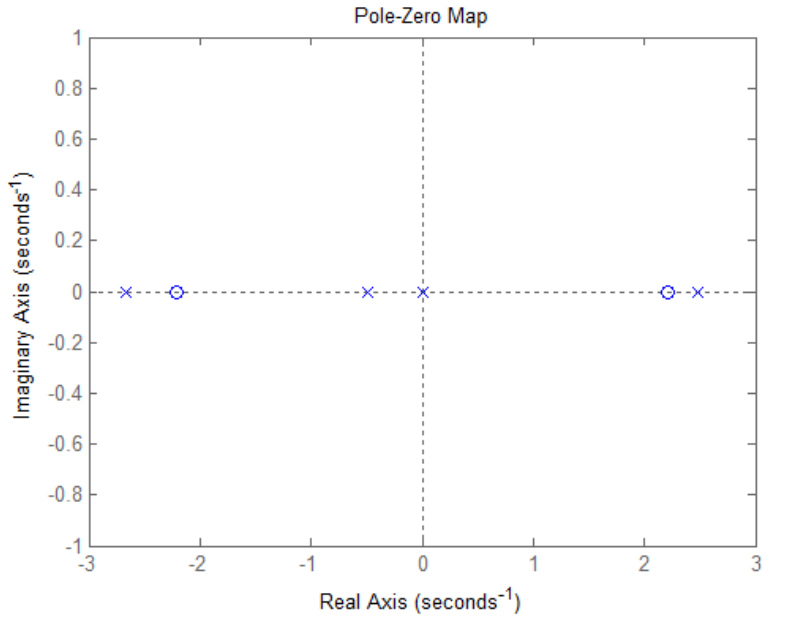
\includegraphics[width=0.7\linewidth]{assets/pole-zero-map}
	\caption{MATLAB-generated pole-zero map of the open loop system $G_{\theta}$ revealing a pole in the right half plane}
	\label{fig:pole-zero-map}
\end{figure}


\subsubsection{Measurement Equation} 
The system's measurement output, which reflects the measured angle, is given by:
\begin{equation}
	{y}(t) = \theta(t) \label{eq:measurement_eq}
\end{equation}
Here, $\mathbf{y}(t)$ denotes the measurement output, which directly corresponds to the system’s angle $\theta(t)$, with no contribution from the gyroscope bias. This measurement model assumes that the system's only observable state is the angle.



\subsubsection{State-space Representation}
The state-space representation of the system is given by:
\begin{equation}
\begin{aligned}
	\underline{\dot{x}}(t) &= \underline{A}.\underline{x}(t) + \underline{B}.\underline{u}(t) \\
	\underline{y}(t) &= \underline{C}.\underline{x}(t) + \underline{D}.\underline{u}(t) \label{eq:state_space_eq}
\end{aligned}
\end{equation}
\begin{itemize}
	\item \textbf{State Vector} $\mathbf{x}(t)$: This vector encapsulates the internal state of the system at time $t$. In this case, it is defined as: 
	\begin{equation}
		\mathbf{x}(t) = \begin{bmatrix} \theta(t) \\ \dot{\theta}(t) \end{bmatrix}
	\end{equation}
	Where $\theta(t)$ represents the measured angle of the system, and $\dot{\theta}_{bias}(t)$ denotes the bias of the gyroscope.
	
	\item \textbf{Input Vector} $\mathbf{u}(t)$: This vector represents the external input given to the system at time $t$. In this case, it is defined as:
	\begin{equation}
		\mathbf{u}(t) = u_{input} 
	\end{equation}
	\item \textbf{State Transition Matrix} $\mathbf{A}$: This matrix describes how the state evolves over time. It is defined as:
\begin{equation}
	\mathbf{A} = \begin{bmatrix}
		0 & 1 \\
		\frac{m_{pend} g l (m_{cart} + m_{pend})}{I_{pend} (m_{cart} + m_{pend}) + m_{cart} m_{pend} l^2} & 0
	\end{bmatrix} \label{eq:state_transition_matrix}
\end{equation}
	The first row indicates that the angle is updated based on its previous value, and the second row shows that the gyroscope bias remains constant in this model.

	\item \textbf{Control Input Matrix} $\mathbf{B}$: This matrix relates the control inputs to the state. In this case, it is defined as:
\begin{equation}
	\mathbf{B} =  \begin{bmatrix}
		0 \\
		\frac{m_{pend} l}{I_{pend} (m_{cart} + m_{pend}) + m_{cart} m_{pend} l^2}
	\end{bmatrix} \label{eq:control_input_matrix}
\end{equation}
	This indicates that there are no direct control inputs affecting the state in this model.
	
	\item \textbf{Measurement Matrix} $\mathbf{C}$: This matrix maps the state vector to the measurement output. It is defined as:
\begin{equation}
	\mathbf{C} = \begin{bmatrix} 1 & 0 \end{bmatrix} \label{eq:measurement_matrix}
\end{equation}
	This means that the measurement output directly reflects the angle, with no contribution from the gyroscope bias.
	
	\item \textbf{Feed-forward Matrix} $\mathbf{D}$: This matrix relates the control input directly to the measurement output. In this case, it is defined as:
\begin{equation}
	\mathbf{D} = 0 \label{eq:feedforward_matrix}
\end{equation}
	This indicates that there is no direct influence of the control input on the measurement output.	

	\item \textbf{Controllability and Observability}: The system is controllable observable if the matrices $S$ and $O$ have full rank.
\begin{equation}
	\mathbf{S} =  \begin{bmatrix} B & AB \end{bmatrix} \label{eq:eq}
\end{equation}

\begin{equation}
	\mathbf{O} =  \begin{bmatrix} C \\ CA \end{bmatrix} \label{eq:eq}
\end{equation}

The rank of $S$ and $O$ confirms that \textbf{the system is controllable and observable} for any positive value of $l$, $I_{pend}$, $m_{cart}$, $m_{pend}$ and $g$.
\end{itemize}

\include{firmware_overview.tex}
\section{Sensor Fusion for Self-Balancing Robot using MPU6050}
\subsection{Introduction}
Self-balancing robots require accurate estimation of their tilt angle for effective control. The MPU6050, a widely used Inertial Measurement Unit (IMU), provides raw accelerometer and gyroscope data. However, due to individual sensor limitations, direct usage of these readings is unreliable. Sensor fusion techniques like the Complementary Filter and Kalman Filter help in obtaining a stable and accurate tilt angle

\subsubsection{Microcontroller}
The ATmega328P (shown in Fig. \ref{fig:ATmega328p}) is a popular microcontroller from Microchip Technology, widely used in embedded systems and electronics projects. With a 16 MHz clock speed, 32 KB of flash memory, 2 KB of SRAM, and 1 KB of EEPROM \cite{atmega_microchip}, the ATmega328P provides ample resources for this projects application. 

The ATMEGA328P is also used in the Arduino Nano (shown in Fig. \ref{fig:arduino_nano}), a widely adopted development board known for its low cost and open-source ecosystem \cite{arduino_nano}. The combination of affordability and extensive community support makes it an ideal choice for rapid prototyping and academic research, ensuring easy integration with various sensors and motor drivers. 

\begin{figure}[H]
	\centering
	\subfloat[ATMEGA328P \cite{atmega_microchip}.]{
		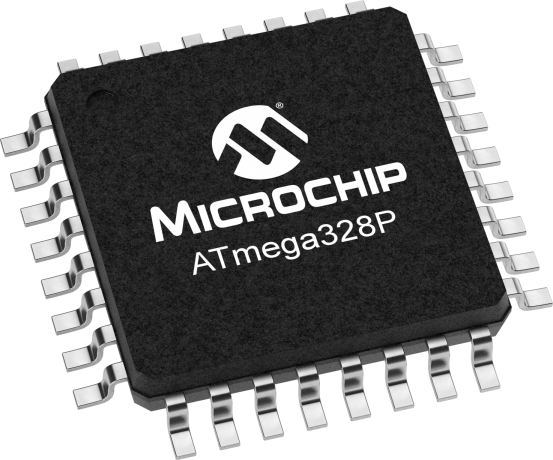
\includegraphics[height=3cm]{assets/ATmega328p.png}
		\label{fig:ATmega328p}
	}
	\qquad
	\subfloat[Arduino Nano \cite{arduino_nano}.]{
	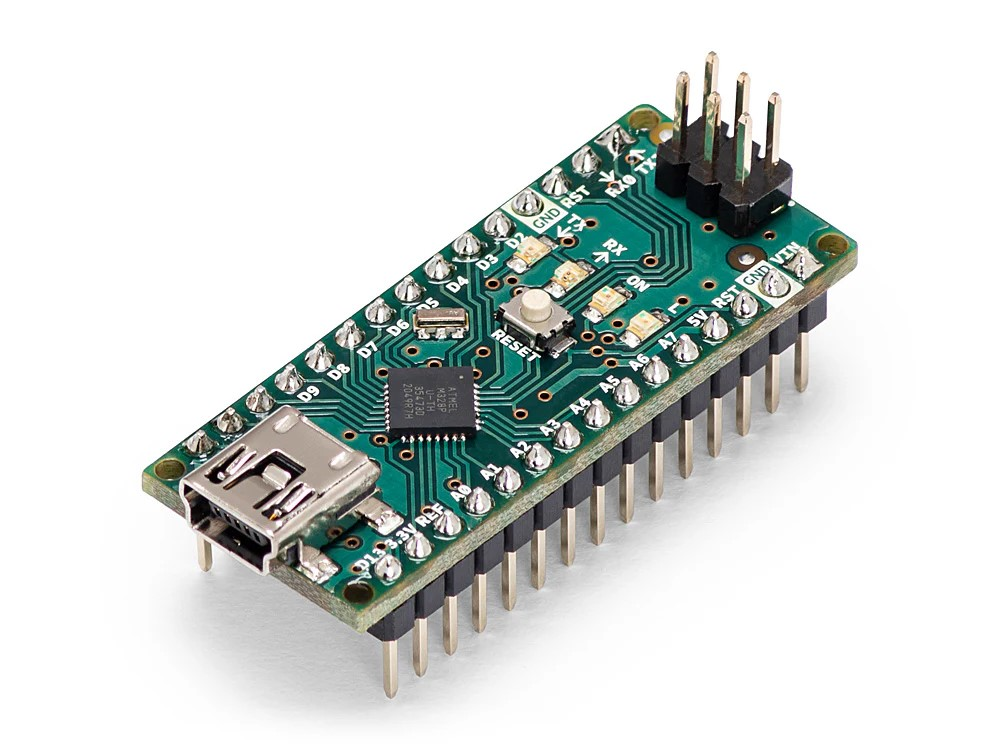
\includegraphics[height=3cm]{assets/arduino_nano.jpg}
	\label{fig:arduino_nano}
	} 
	\label{fig:ATmega328p_and_arduino_nano}
	\caption{}
\end{figure}

\subsubsection{Inertial Measuring Unit}
The MPU6050 is a widely used six-axis sensor that integrates a three-axis gyroscope and a three-axis accelerometer on a single chip, making it essential for motion tracking and stabilization applications (shown in Fig. \ref{fig:mpu-6050}). Its compact design and built-in Digital Motion Processor (DMP) enable real-time processing of sensor data, which is crucial for robotics, drones, and wearable devices.
In applications like self-balancing robots, it provides accurate orientation and acceleration data necessary for maintaining stability. 

\begin{figure}[H]
	\centering
	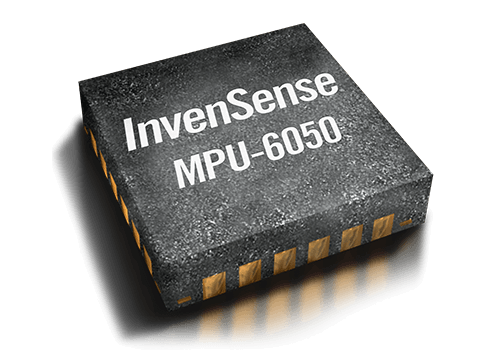
\includegraphics[height=3cm]{assets/mpu-6050.png}
	\caption{MPU-6050 \cite{mpu6050}.}
	\label{fig:mpu-6050}
\end{figure}


\subsection{Working of MPU6050}
The MPU6050 is a 6-axis IMU that provides:
\begin{itemize}
	\item Accelerometer Data: Measures acceleration in X, Y, and Z axes. It helps in estimating tilt based on gravitational force.
	\item Gyroscope Data: Measures angular velocity around X, Y, and Z axes. Integration of gyroscope readings over time provides the tilt angle.
\end{itemize}

\subsubsection{Reading Raw Sensor Data}
The \texttt{read\_mpu\_6050\_data()} function reads raw data from the MPU6050 sensor:
\begin{itemize}
	\item It requests 14 bytes of data from the sensor, covering the accelerometer, gyroscope, and temperature sensor readings.
	\item The data is stored in respective variables after combining the high and low bytes. 
	\item If data retrieval fails, an error message is displayed.
\end{itemize}
\begin{lstlisting}[style=cppstyle2]
void mpu6050Base::read_mpu_6050_data() {
	Wire.beginTransmission(mpu6050_addr);
	Wire.write(0x3B);
	Wire.endTransmission();
	Wire.requestFrom(mpu6050_addr, (uint8_t)14);
	
	if (Wire.available() >= 14) {
		acc_x = Wire.read() << 8 | Wire.read();
		acc_y = Wire.read() << 8 | Wire.read();
		acc_z = Wire.read() << 8 | Wire.read();
		temperature = Wire.read() << 8 | Wire.read();
		gyro_x = Wire.read() << 8 | Wire.read();
		gyro_y = Wire.read() << 8 | Wire.read();
		gyro_z = Wire.read() << 8 | Wire.read();
	} else {
		ERROR_PRINT("Data cannot be read from MPU6050!");
	}
	
}
\end{lstlisting}

\subsubsection{Issues with Raw Sensor Data}
\begin{itemize}
\item \textbf{Accelerometer Noise}: While providing an absolute angle reference, accelerometer readings are noisy and susceptible to external forces.
\item \textbf{Gyroscope Drift}: Over time, integration errors cause drift, leading to inaccurate angle estimation.
To overcome these issues, sensor fusion techniques are applied.
\end{itemize}


\subsection{Complementary Filter}
The complementary filter is a simple yet effective method for sensor fusion \cite{rabbany_design_2021} \cite{10193276} \cite{1174486}. It blends high-frequency data from the gyroscope with low-frequency data from the accelerometer:

\subsubsection{Mathematical Model}
Raw accelerometer readings $A_y$ and $Az$ can be used to calculate tilt angle using following equation:
\begin{equation}
\theta_{acc} = \text{arctan} \left(A_y/Az  \right) \label{eq:eq}
\end{equation}
Similarly, using raw angular velocity data from the gyroscope $\omega_{x}$,
\begin{equation}
	\begin{aligned}
		\dot{\theta}_{gyro}(t) &= - \omega_{x,bias}(t) \\ \label{eq:state_eq_1}
		\dot{\omega}_{x,bias}(t) &= 0
	\end{aligned}
\end{equation}
In these equations, $\theta(t)$ represents the measured angle of the system, and $\omega_{\text{gyro,bias}}(t)$ represents the bias of the gyroscope. The first equation models how the angle evolves over time, influenced by the constant gyroscope bias. The second equation indicates that the gyroscope bias remains constant over time. The sampling time interval $\Delta t$ and previous angle value $\theta_{previous}$ can be used to calculate tilt angle using following equation:
\begin{equation}
\theta_{gyro} = \theta_{previous, gyro} + \omega_{gyro} \Delta t \label{eq:eq}
\end{equation}
Then the final estimated angle $\theta_{estimate}$ is calculated as:
\begin{equation}
	\theta_{estimate} = \alpha \ \theta_{gyro} + (1 - \alpha) \ \theta_{acc} \label{eq:eq}
\end{equation}
Where $\alpha$ is the filter coefficient, $\omega$ is the angular velocity from the gyroscope, and $\theta_{acc}$ is the angle from the accelerometer.

\subsubsection{Initial Calibration}
The \texttt{init()} function is responsible for initializing the MPU6050 sensor and performing gyroscope calibration:
\begin{itemize}
	\item The I2C communication is established with the sensor, and an acknowledgment is checked to ensure proper connection.
	\item The function sets up the MPU6050 registers using \texttt{setup\_mpu\_6050\_registers()}, configuring the power management and sensitivity ranges for both the accelerometer and gyroscope.
	\item Gyroscope calibration is performed by collecting multiple readings and averaging them to calculate offsets for the X, Y, and Z axes. These offsets help reduce sensor drift.
\end{itemize}

\begin{lstlisting}[style=cppstyle2]
void mpu6050Base::init() {
	Wire.beginTransmission(mpu6050_addr);
	if (Wire.endTransmission() != 0) {
		ERROR_PRINT("MPU6050 not connected!");
		return;
	}
	setup_mpu_6050_registers();
	
	for (int i = 0; i < CALIBRATION_SAMPLES; i++) {
		read_mpu_6050_data();
		gyro_x_cal += gyro_x;
		gyro_y_cal += gyro_y;
		gyro_z_cal += gyro_z;
		delay(3);
	}
	gyro_x_cal /= CALIBRATION_SAMPLES;
	gyro_y_cal /= CALIBRATION_SAMPLES;
	gyro_z_cal /= CALIBRATION_SAMPLES;
}
\end{lstlisting}

\subsubsection{Calculating Angles}
The \texttt{calculate()} function processes raw sensor data to determine pitch and roll angles:
\begin{itemize}
	\item Gyroscope readings are corrected using calibration offsets to remove bias.
	\item Angular velocity is integrated over time to estimate orientation changes.
	\item The accelerometer-derived angles are computed from the total acceleration vector using trigonometric transformations.
	\item A complementary filter is applied to blend gyroscope and accelerometer readings, mitigating drift and noise while enhancing stability.
\end{itemize}

\begin{lstlisting}[style=cppstyle2]
void mpu6050Base::calculate() {
	read_mpu_6050_data();
	
	gyro_x -= gyro_x_cal;
	gyro_y -= gyro_y_cal;
	gyro_z -= gyro_z_cal;
	
	angle_pitch += gyro_x * 0.0000611;
	angle_roll += gyro_y * 0.0000611;
	
	angle_pitch += angle_roll * sin(gyro_z * 0.000001066);
	angle_roll -= angle_pitch * sin(gyro_z * 0.000001066);
	
	acc_total_vector = sqrt((acc_x * acc_x) + (acc_y * acc_y) + (acc_z * acc_z));
	
	angle_pitch_acc = asin((float)acc_y / acc_total_vector) * 57.296;
	angle_roll_acc = asin((float)acc_x / acc_total_vector) * -57.296;
	
	if (set_gyro_angles) {
		angle_pitch = angle_pitch * 0.9996 + angle_pitch_acc * 0.0004;
		angle_roll = angle_roll * 0.9996 + angle_roll_acc * 0.0004;
	} else {
		angle_pitch = angle_pitch_acc;
		angle_roll = angle_roll_acc;
		set_gyro_angles = true;
	}
	
	angle_pitch_output = angle_pitch_output * 0.9 + angle_pitch * 0.1;
	angle_roll_output = angle_roll_output * 0.9 + angle_roll * 0.1;
	
}
\end{lstlisting}


\subsubsection{Results}

\begin{figure}[H]
	\centering
	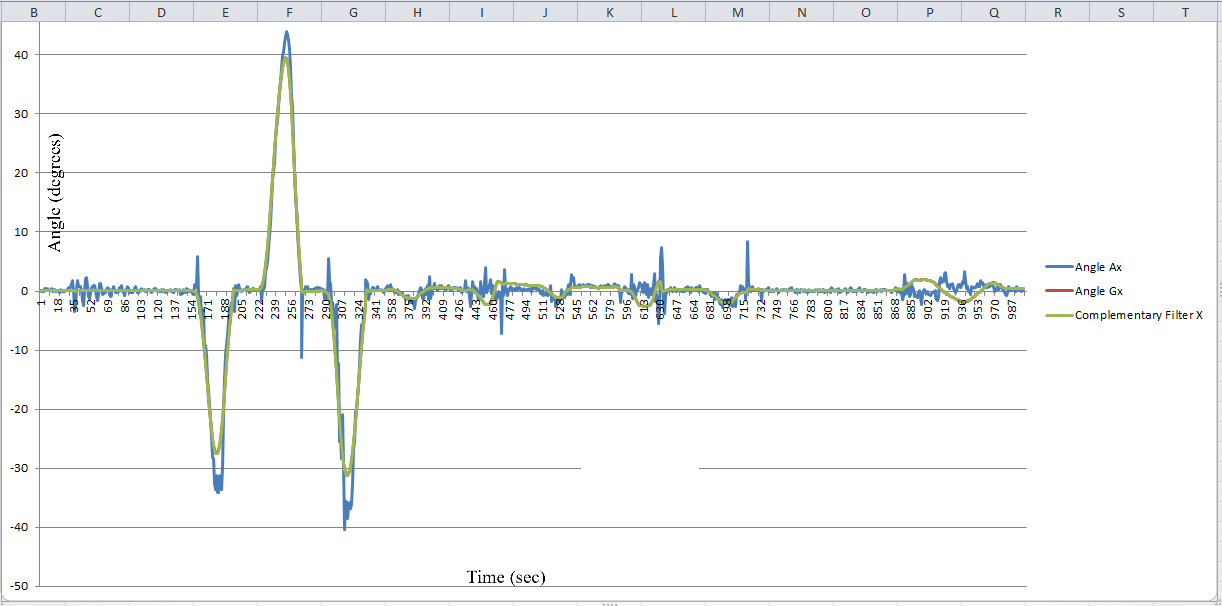
\includegraphics[height=8cm]{assets/compl_filter_0.9.png}
	\caption{Pitch angle caluclated using a complementary filter with $\omega = 0.9$.}
	\label{fig:battery}
\end{figure}


\subsection{Extended Kalman Filter (EKF)}
The Kalman filter (KF) provides a more sophisticated approach, estimating the true state of the system by minimizing the mean of the squared error. It involves prediction and update steps. However,  assumes that both the process and measurement models are linear. However, many real-world systems, such as robotic motion and sensor fusion, exhibit inherent nonlinearities. When linearization is not feasible, the standard KF becomes inaccurate. 

To address this limitation, the Extended Kalman Filter (EKF) extends the KF to nonlinear systems by employing a first-order Taylor series expansion. This method approximates the nonlinear system dynamics and measurement models with locally linearized representations, allowing the filter to be applied in scenarios where exact linearization is not feasible.

The EKF is an extension of the Kalman Filter for nonlinear systems, utilizing first-order Taylor series expansion to linearize process and measurement models. EKF maintains a Gaussian belief over the state, updating it through a prediction-correction cycle. The Jacobian matrices of the system dynamics and measurement functions are used to approximate state transitions and measurement updates. Its advantages include handling nonlinearities, fusing multi-sensor data, and improving estimation accuracy in noisy environments. 

\subsubsection{General State Equation}
For non-linear system, with Stochastic disturbances:
\begin{equation}
\begin{aligned}
	\dot{\underline{x}}(t) &= f\left( \underline{x}(t), \underline{u}(t) \right) + \underline{d}(t) \\
	\underline{y}(t) &= h\left( \underline{x}(t) \right) + \underline{n}(t)
\end{aligned}
\end{equation}
where,
\begin{itemize}
	\item $ \dot{\underline{x}}(t) $: This represents the time derivative of the state vector $ \underline{x}(t) $, indicating how the state evolves over time.
	\item $ f $: This is a nonlinear function that describes the system dynamics, taking the current state $ \underline{x}(t) $ and the control input $ \underline{u}(t) $ as arguments. It captures how the state changes based on the current state and control inputs.
	\item $ \underline{d}(t) $: This term represents stochastic disturbances (or process noise) affecting the state dynamics, typically modeled as a zero-mean Gaussian noise.
	\item $ y(t) $: This is the measurement vector at time $ t $, representing the observed outputs of the system. It is the data collected from sensors or measurement devices.
	\item $ h $: This is a nonlinear measurement function that maps the true state vector $ \underline{x}(t) $ to the measurement space. It describes how the state influences the measurements. The function $ h $ can be complex and may involve various transformations of the state variables.
	\item $ n(t) $: This term represents measurement noise, which is also typically modeled as zero-mean Gaussian noise. It accounts for inaccuracies in the measurements due to sensor errors, environmental conditions, or other random factors that can affect the observed data.
\end{itemize}

\subsubsection{State Estimation}
For a non-linear system the state form is as follows,
\begin{equation}
\begin{aligned}
	\dot{\hat{\underline{x}}}(t) &= f\left( \underline{\hat{x}}(t), \underline{u}(t) \right) + \underline{K}\left( y(t) - \hat{y}(t) \right) \\
	\hat{y}(t) &= h\left( \underline{\hat{x}}(t) \right)  \label{eq:eq}
\end{aligned}
\end{equation}
The Kalman gain $\underline{K}$ is computed to optimally balance estimation uncertainty and measurement noise. To achieve this, the system is first linearized around the current state estimate by computing the Jacobians of the process and measurement models. To linearize the system around the current state estimate, the Jacobian matrices, which represent the first-order partial derivatives of the nonlinear functions, are computed as follows:
\begin{equation}
\underline{A}(t) = \frac{\mathrm{d}f}{\mathrm{d}\underline{x}} \bigg|_{\underline{\hat{x}}(t), \underline{u}(t)} \quad \text{and} \quad
\underline{C}(t) = \frac{\mathrm{d}h}{\mathrm{d}\underline{x}} \bigg|_{\underline{\hat{x}}(t)}  \label{eq:eq}
\end{equation}
where $\underline{A}(t)$ represents the partial derivatives of the state dynamics function $f$ and $\underline{C}(t)$ represents the partial derivatives of the measurement function $h$.
\begin{figure}[h]
	\centering
	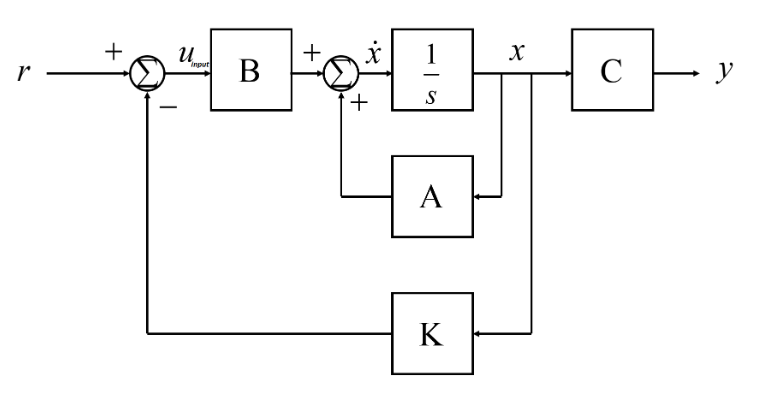
\includegraphics[height=5cm]{assets/block_representation_kalman_filter.png}
	\caption{Block representation of state space system showing the system matrices $A$, $B$ and $C$ as well as the gain matrix $K$.}
	\label{fig:block_representation_kalman_filter}
\end{figure}
\subsubsection{Covraince Matrix}
The evolution of the state estimation covariance matrix follows the continuous-time Riccati equation, given by:
\begin{equation}
\dot{P}(t) = \underline{A}(t) P(t) + P(t) \underline{A}^T(t) + Q - P(t) \underline{C}^T(t) R^{-1} \underline{C}(t) P(t)  \label{eq:eq}
\end{equation}
Where, 
\begin{itemize}
	\item $\dot{P}(t)$: his represents the time derivative of the covariance matrix $\dot{P}(t)$, which quantifies the uncertainty in the state estimate over time.
	\item $\underline{A}(t)$: This is the state transition matrix, which describes how the state evolves from one time step to the next.
	\item $Q$: This is the process noise covariance matrix, representing the uncertainty in the process model.
	\item $\underline{C}(t)$: This is the measurement matrix, which relates the state to the measurements.
	\item $R$: This is the measurement noise covariance matrix, representing the uncertainty in the measurements.
\end{itemize}
The Kalman filter is initialized with an initial covariance matrix:
\begin{equation}
	P(0) = \mathbf{E}(\Delta\underline{x}(0) \Delta\underline{x}^T(0))  \label{eq:eq}
\end{equation}
The optimal Kalman gain, balancing estimation uncertainty and measurement noise, is given by:

\begin{equation} \underline{K}(t) = P(t) \underline{C}^T R^{-1} \end{equation}
The time-discrete Kalman filter state update equations are:
\begin{equation}
	\begin{aligned}
		\underline{x}_{k} &= \underline{A} \underline{x}_{k-1} + \underline{B} \underline{u}_{k} + \underline{d}_{k-1} \\
		\underline{y}_{k} &= \underline{C} \underline{x}_{k} + \underline{n}_{k}  \label{eq:eq}
	\end{aligned}
\end{equation}
where $\underline{x}_k$ is the state vector, $\underline{B}$ the control input matrix, and $\underline{y}_k$ the measurement vector. The discrete state-space representation is:
\begin{equation}
	\begin{aligned}
		\underline{\dot{x}}(t) = \underline{A}.\underline{x}(t) + \underline{B}.\underline{u}(t) \\
		\underline{y}(t) = \underline{C}.\underline{x}(t) + \underline{D}.\underline{u}(t)  \label{eq:eq}
	\end{aligned}
\end{equation}
The state covariance matrix is:
\begin{equation}
	\mathbf{P}_k = \begin{bmatrix} P_{00} & P_{01} \\ P_{10} & P_{11} \end{bmatrix}  \label{eq:eq}
\end{equation}
where $P_{00}$ represents uncertainty in the angle estimate and $P_{11}$ in gyroscope bias. The Kalman gain is computed as:
\begin{equation}
	\begin{aligned}
		\underline{K}_{k} &= \underline{P}_{k}^- \ \underline{C}^T ( \underline{C} \ \underline{P}_{k}^-\ \underline{C}^T  +\underline{R})^{-1} \\ \\
		\mathbf{K}_k &= \begin{bmatrix} \frac{ P_{00} }{ P_{00}  
				+ R_{angle}} \\ \frac{ P_{10} }{ P_{00}  
				+ R_{angle}} \end{bmatrix}
	\end{aligned}  \label{eq:eq}
\end{equation}
Following the prediction step, the measurement update step refines the state estimate using the Kalman gain, which is derived to minimize the posterior estimation error covariance (see Appendix \ref{appendix:B} for detailed calculations):
\begin{equation}
	\begin{aligned}
		\underline{P}_{k} &= \ (\underline{I} - \underline{K}_{k} \ \underline{C}) \ \underline{P}_{k}^- \label{eq:eq}
	\end{aligned}
\end{equation}


\subsection{Software Implementation of EKF}
For the implementation of the Extended Kalman Filter (EKF), we utilized the Kalman filter library developed by Kristian Lauszus~\cite{github_kalman_filter}. This library was modified in accordance with the GNU General Public License to meet the specific requirements of our project.
\begin{lstlisting}[style=cppstyle2]
#include <Arduino.h>

class KalmanFilter {
 private:
  float m_dt, m_Q_angle, m_Q_gyro, m_R_angle, m_C_0;
  float q_bias = 0, angle_err = 0;
  float P[2][2] = {{1, 0}, {0, 1}}; // Covariance matrix
  float K_0 = 0, K_1 = 0;

 public:
  float angle = 0;

KalmanFilter(float dt, float Q_angle, float Q_gyro, float R_angle, float C_0)
: m_dt(dt), m_Q_angle(Q_angle), m_Q_gyro(Q_gyro), m_R_angle(R_angle), m_C_0(C_0) {}

float getAngle(float measured_angle, float measured_gyro) {
	// Predict
	angle += (measured_gyro - q_bias) * m_dt;
	angle_err = measured_angle - angle;
	
	// Update covariance matrix
	P[0][0] += m_Q_angle - P[0][1] - P[1][0];
	P[0][1] -= P[1][1];
	P[1][0] -= P[1][1];
	P[1][1] += m_Q_gyro;
	
	// Compute Kalman gain
	float E = m_R_angle + m_C_0 * P[0][0];
	K_0 = (m_C_0 * P[0][0]) / E;
	K_1 = (m_C_0 * P[1][0]) / E;
	
	// Update state
	angle += K_0 * angle_err;
	q_bias += K_1 * angle_err;
	
	// Update covariance matrix
	float C0_P00 = m_C_0 * P[0][0];
	P[0][0] -= K_0 * C0_P00;
	P[0][1] -= K_0 * P[0][1];
	P[1][0] -= K_1 * P[0][0];
	P[1][1] -= K_1 * P[0][1];
	
		return angle;
	}
};
\end{lstlisting}
\subsection{PID Controller}\label{section:pid_controller}
\subsubsection{Basic Structure}
The PID controller generates a control signal $u(t)$ based on the error signal $e(t)$, which is the difference between the desired setpoint and the measured process variable (see Fig. \ref{fig:control-loop-block-diagram}). The control signal is computed as:

\begin{equation}
	u(t) = K_p e(t) + K_i \int_0^t e(\tau)d\tau + K_d \frac{d}{dt}e(t)
\end{equation}

Where:
\begin{itemize}
	\item $u(t)$: Control signal applied to the system.
	\item $e(t)$: Error signal, representing the deviation from the setpoint.
	\item $K_p$: Proportional gain, which responds to the current error.
	\item $K_i$: Integral gain, which addresses accumulated past errors.
	\item $K_d$: Derivative gain, which predicts future error trends based on the rate of change.
\end{itemize}

\subsubsection{Discrete Time Implementation}
For digital implementation, the continuous-time PID equation is discretized to suit microcontroller-based systems. The discrete-time PID control signal u[n]u[n] is calculated as:

\begin{equation}
	u[n] = K_p e[n] + K_i T_s \sum_{k=0}^n e[k] + K_d \frac{e[n] - e[n-1]}{T_s}
\end{equation}

where:
\begin{itemize}
	\item $T_s$: Sampling period, representing the time interval between consecutive control updates.
	\item $e[n]$: Error signal at the nn-th sampling instant.
	\item $u[n]$: Control signal at the nn-th sampling instant.
\end{itemize}
This formulation ensures compatibility with real-time embedded systems while maintaining control precision.


\subsection{Tuning Methodology}
The Ziegler-Nichols method is a widely used and systematic approach for tuning PID controllers. It provides a reliable framework for determining initial controller parameters, which can then be fine-tuned for optimal performance. The method involves inducing controlled oscillations in the system to identify critical parameters, which are then used to calculate the proportional, integral, and derivative gains.
\subsubsection{Ziegler-Nichols Method}
The Ziegler-Nichols tuning procedure consists of the following steps:
\begin{enumerate}
	\item \textbf{Initialize Parameters}: Set the integral gain \( K_i \) and derivative gain \( K_d \)to zero, leaving only the proportional gain \( K_p \) active.
	\item \textbf{Induce Oscillations}: Gradually increase \( K_p \) until the system exhibits sustained oscillations. At this point, the system is at the threshold of stability, and the proportional gain is referred to as the ultimate gain \( K_u \). The period of these oscillations is denoted as \( T_u \).
	\item \textbf{Record Critical Values}: Note the values of \( K_u \) and \( T_u \), as they are essential for calculating the final PID parameters.
	\item \textbf{Calculate PID Gains:} Using the recorded values, compute the PID parameters as follows:
	\begin{equation}
		\begin{aligned}
			K_p &= 0 . 6K_u \\
			T_i &= 0 . 5T_u \\
			T_d &= 0 . 125T_u  \label{eq:eq}
		\end{aligned}
	\end{equation}
	Here, \( T_i \) and \( T_d \) represent the integral and derivative time constants, respectively. These values are then used to determine the integral and derivative gains:
	\begin{equation}
		\begin{aligned}
			K_i = \frac{K_p}{T_i} \quad \text{and} \quad K_d = K_p \cdot T_d.  \label{eq:eq}
		\end{aligned}
	\end{equation}
\end{enumerate}

This method provides a robust starting point for achieving stable control. However, it is important to note that the Ziegler-Nichols method may require additional fine-tuning to account for system-specific dynamics and performance requirements. The calculated parameters serve as an initial baseline, which can be further optimized through iterative testing and adjustment.


\subsubsection{Practical Tuning Guidelines}
In addition to the Ziegler-Nichols method, practical tuning guidelines were applied to refine the controller performance:

\begin{itemize}
	\item Start with a small proportional gain $K_p$ (e.g. $K_p$ = 10) to avoid instability.
	\item Introduce the derivative term $K_d$ to dampen oscillations, typically setting $K_d = 0 . 1K_p$.
	\item  Fine-tune $K_p$, $K_i$, and $K_d$ iteratively to achieve optimal stability and responsiveness.
\end{itemize}


\subsection{Cascaded PID Control Strategy}
To optimize system performance and resource utilization, the control loop employs a cascaded PID strategy:
\begin{itemize}
	\item \textbf{Pitch Control}: Updated at the highest frequency (e.g., every control cycle) to ensure rapid response to changes in the robot's tilt and maintain balance.
	\item \textbf{Yaw and Position Control}: Updated at a lower frequency (e.g., every 8th cycle) to reduce computational load while still providing adequate motion control.
\end{itemize}

This approach prioritizes critical tasks (e.g., maintaining balance) while efficiently managing system resources, ensuring robust and stable operation. A simplified block diagram for a cascaded PID controller is shown in Fig.~\ref{fig:control-loop}

\begin{figure}[H]
	\centering
	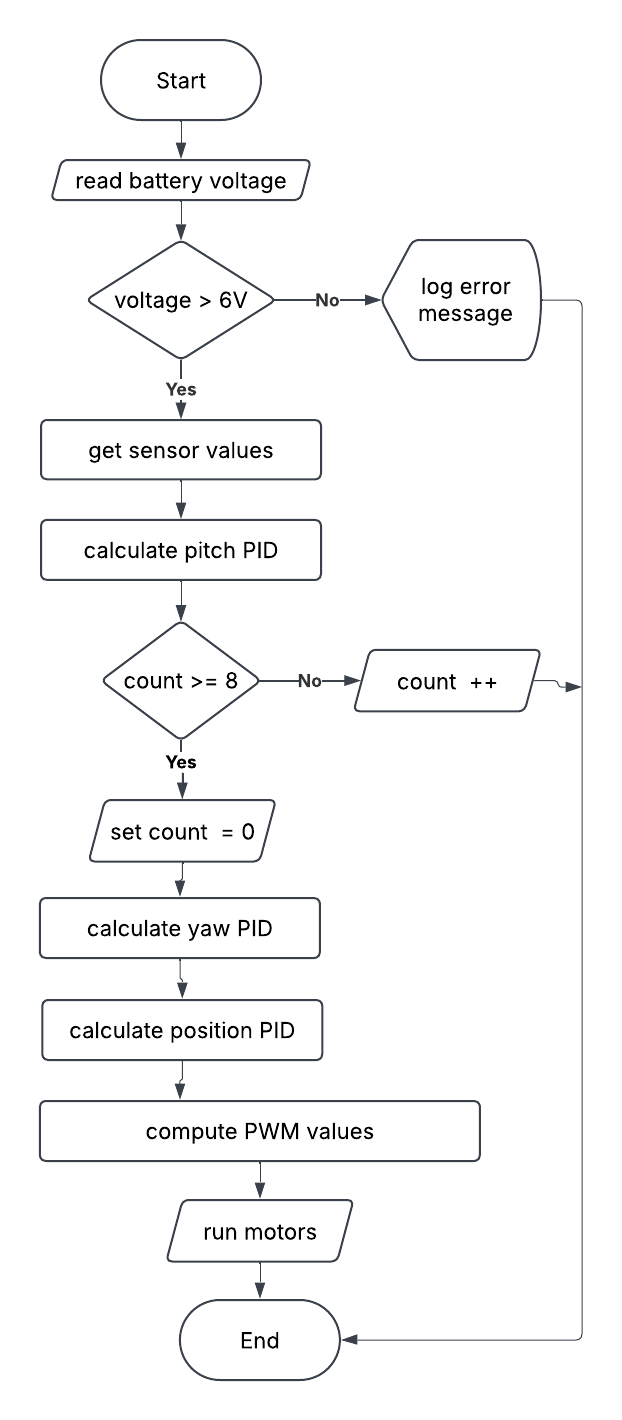
\includegraphics[width=0.5\linewidth]{assets/control_loop_diagram.png}
	\caption{A simplified block diagram of the cascaded control loop used. }
	\label{fig:control-loop}
\end{figure}

\subsubsection{Pitch PID Control:}
The pitch control loop ensures the robot maintains its upright position. The primary objective of the pitch controller is to minimize the deviation of the robot's pitch angle from a set-point, which is ideally zero degrees (i.e., upright). The pitch control output is calculated using the PD algorithm, where the error is the difference between the current pitch angle and the desired pitch angle. 
\begin{equation}
	\tau_{\theta,pid} = K_{p\theta}({\theta_{desired} - \theta_{measured}}) + K_{d\theta}\frac{d}{dt}(\theta_{desired} - \theta_{measured})
\end{equation}

Below is its code implementation:
\begin{lstlisting}[style=cppstyle2]
	inline void runPitchControl() {
		pitch_pid_output = (kp_balance * (kalman.angle - 0)) + (kd_balance * gyro_x);
	}
\end{lstlisting}

The final results are shown in Fig.~\ref{fig:pid_position_kp_55_kd_1_25}.
\begin{figure}[H]
	\centering
	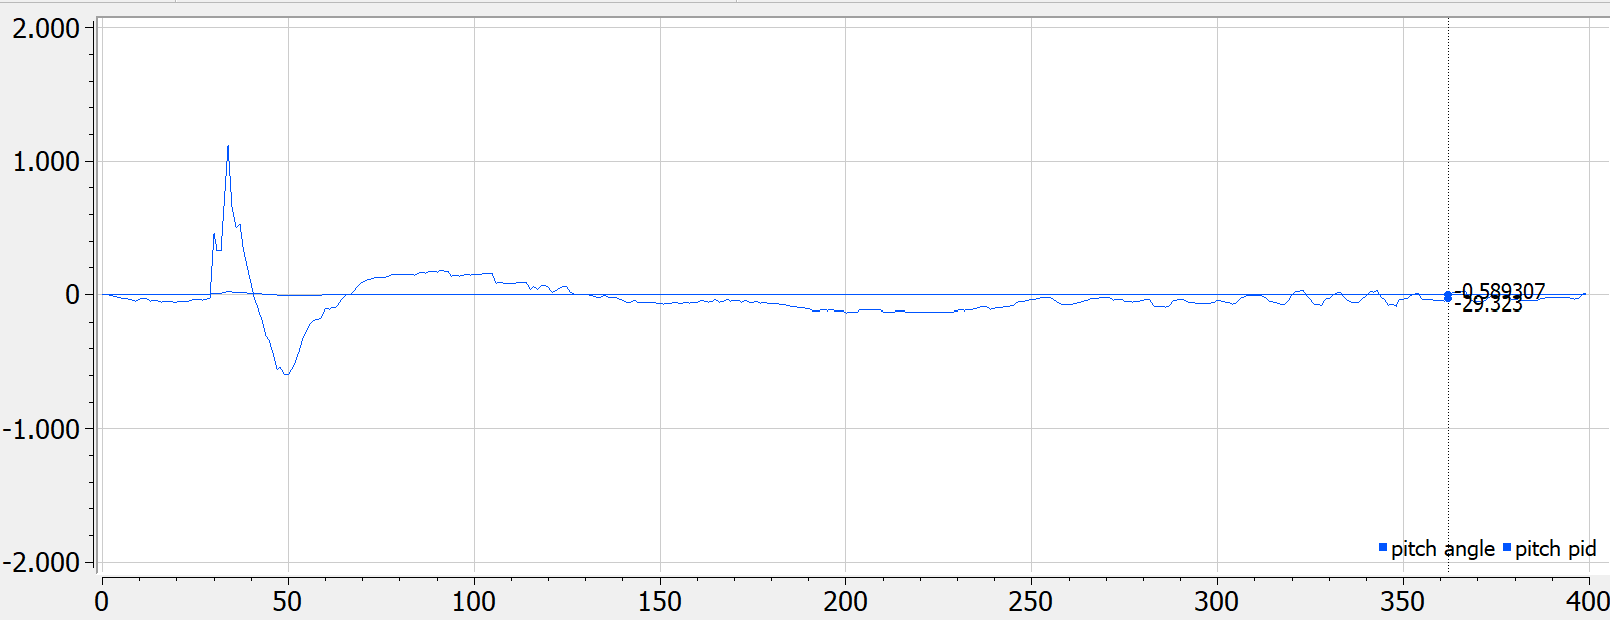
\includegraphics[width=0.8\linewidth]{assets/pid_pitch_kp_55_kd_1_25.png}
	\caption{Pitch angle control system response at $K_{p\theta}$ = 55 and $K_{d\theta}$ = 1.25. The data was recorded at baud rate of 115200.}
	\label{fig:pid_position_kp_55_kd_1_25}
\end{figure}

\textbf{Eliminating Jitter}:
Once the system reaches stability, it begins to exhibit jitter (i.e. small, rapid fluctuations in the control output), as observed in the PID output between data points 250 and 400 in Fig.~\ref{fig:pid_position_kp_55_kd_1_25}. This jitter arises due to the high sensitivity of the derivative gain ($K_{d\theta}$) to fluctuations in the gyroscope readings ($\dot{\theta}$). While reducing $K_{d\theta}$ mitigates the jitter, it also diminishes the system's ability to dampen oscillations, leading to excessive overshoot and potential instability. Fig.~\ref{fig:pid_position_overshoot} illustrates the system's response when using $K_{p\theta}$ = 55 and $K_{d\theta}$ = 0.75 where significant overshoot is evident.

\begin{figure}[H]
	\centering
	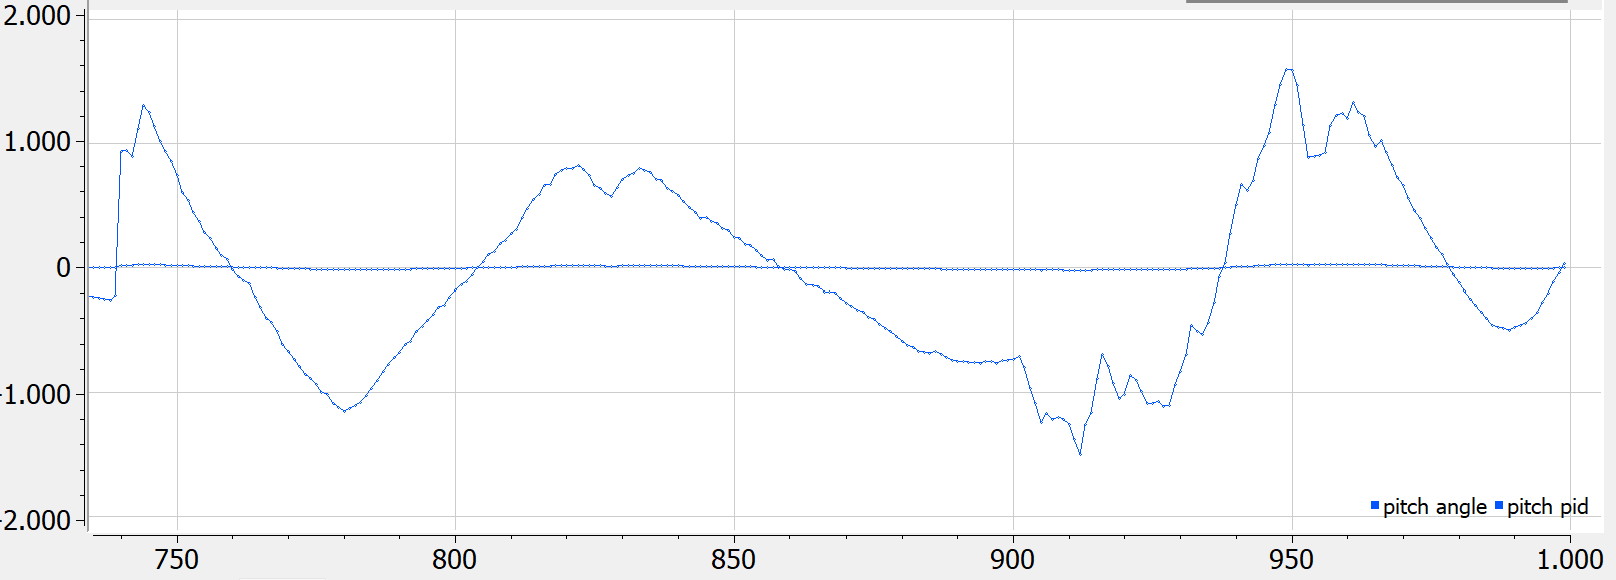
\includegraphics[width=0.7\linewidth]{assets/pid_pitch_overshoot.png}
	\caption{Pitch angle control system response at $K_{p\theta}$ = 55 and $K_{d\theta}$ = 0.75. Data recorded at baud rate of 115200.}
	\label{fig:pid_position_overshoot}
\end{figure}

To address this issue, an \textbf{adaptive derivative gain approach} is implemented, where $K_{d\theta}$ is adjusted dynamically based on the pitch angle of the robot. When the absolute pitch angle exceeds a predefined threshold, a higher derivative gain is used to provide stronger correction, while a lower gain is applied for small angles to minimize jitter. The corresponding implementation is as follows:
\begin{lstlisting}[style=cppstyle2]
	if (pitch_angle > 8) { kd_balance = kd_balance_large_angle; }
	else { kd_balance = kd_balance_small_angle; }
	
	inline void runPitchControl() {
		pitch_pid_output = (kp_balance * (kalman.angle - 0)) + (kd_balance * gyro_x);
	}
\end{lstlisting}

This adaptive control strategy effectively stabilizes the system while reducing excessive oscillations. Fig.~\ref{fig:pid_position_combined} presents the improved system response, demonstrating a smoother transition and enhanced overall stability.
\begin{figure}[H]
	\centering
	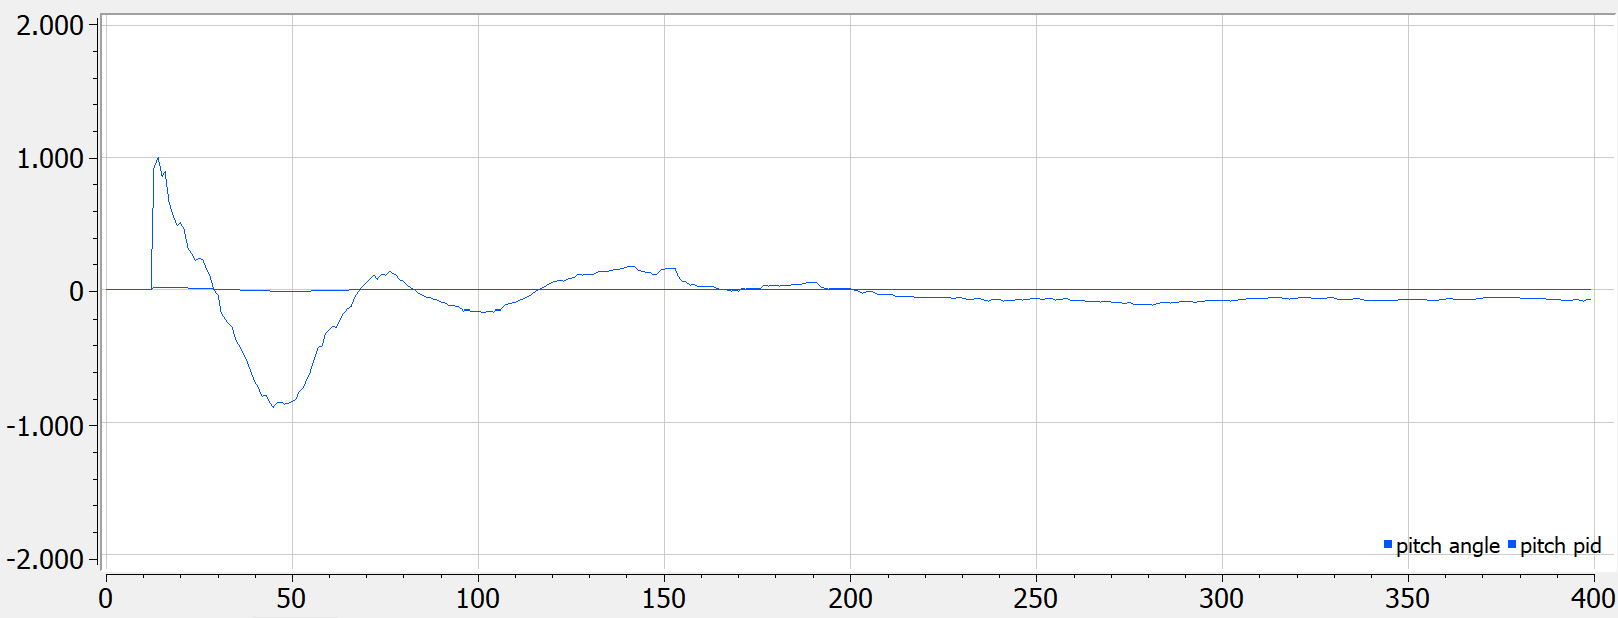
\includegraphics[width=0.8\linewidth]{assets/pid_pitch_combined.png}
	\caption{Pitch angle control system response. The data was recorded at baud rate of 115200.}
	\label{fig:pid_position_combined}
\end{figure}


\subsubsection{Yaw Control:}
Yaw control is responsible for controlling the robot's rotational movement around its vertical axis. The yaw PID controller computes the control output based on the robot's angular velocity, which is measured by the gyroscope along the z-axis. 
\begin{equation}
	\tau_{\phi,pid} = K_{p\phi}(\phi_{desired} - \phi_{measured}) + K_{d\phi}\frac{d}{dt}(\phi_{desired} - \phi_{measured})
\end{equation}

Below is its code implementation:
\begin{lstlisting}[style=cppstyle2]
	inline void runYawControl(){
		float delta_yaw_angle = yaw_angle_degrees - desired_yaw_angle;
		yaw_pid_output = (kp_turn * delta_yaw_angle) + (kd_turn * gyro_z);
	}
\end{lstlisting}

The yaw control adjusts the motor speeds to achieve the desired angle, ensuring the robot maintains a stable heading. Fig.~\ref{fig:pid_yaw} illustrates the system's response with \(K_{p\phi}\) = 2.5 and $K_{i\phi}$ = 0.5 when transitioning from an initial angle of $-20 \ deg$ to final angle of $+20 \ deg$.
\begin{figure}[H]
	\centering
	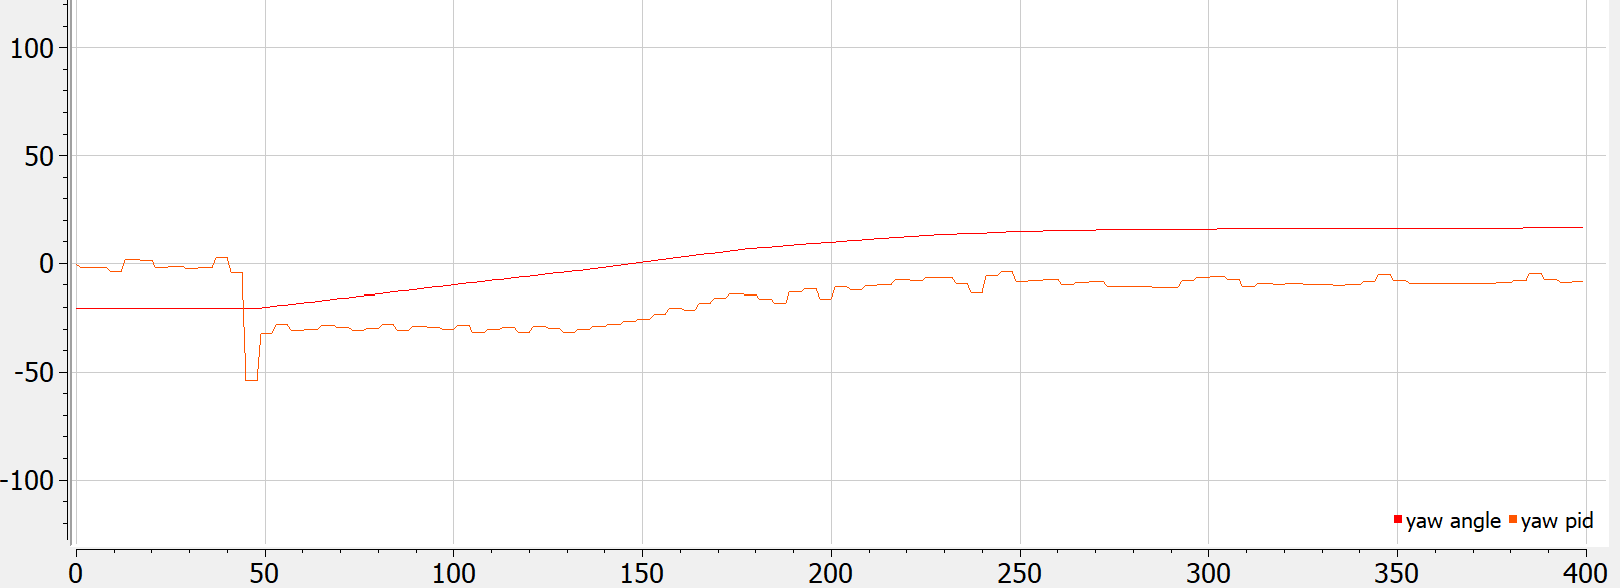
\includegraphics[width=0.8\linewidth]{assets/pid_yaw_kp_2_5_kd_0_5_target_20_deg.png}
	\caption{Yaw angle control system response at \(K_p\) = 2.5 and $K_i$ = 0.5 for an angle transition from $-20 \ deg$ to $+20 \ deg$. The data was recorded at baud rate of 115200.}
	\label{fig:pid_yaw}
\end{figure}

\subsubsection{Position Control:}
Position control is implemented to ensure the robot moves smoothly and accurately along a path or to a target location. The encoder feedback from the left and right wheels is used to calculate the robot's displacement and speed. The position PID controller adjusts the motor speeds to minimize the error in position and velocity.
\begin{equation}
	\tau_{x,pid} = K_{px}(x_{desired} - x_{measured}) + K_{dx}\frac{d}{dt}(x_{desired} - x_{measured})
\end{equation}

Below is its code implementation:
\begin{lstlisting}[style=cppstyle2]
	inline void runPositionControl(){
		position_pid_output = - (kp_position * (current_position - move_to_position)) - (kd_position * encoder_speed_filtered);
	}
\end{lstlisting}

The position controller continuously adjusts motor speeds to reduce position error while maintaining a stable heading. Fig.~\ref{fig:pid_postition} presents the system's response when \(K_{px}\) = 0.26 and $K_{dx}$ = 20 when moving from relative distance of $-60 \ cm$ to $+30 \ cm$.
\begin{figure}[H]
	\centering
	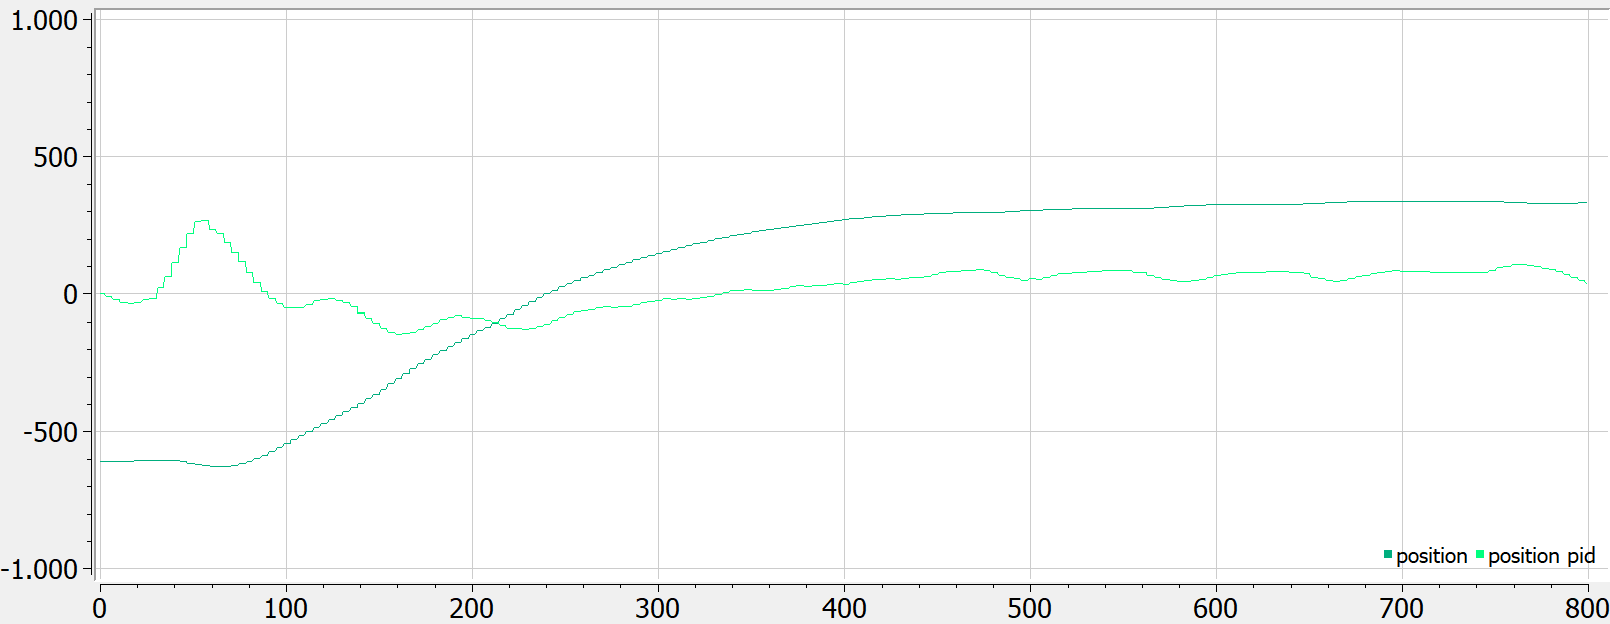
\includegraphics[width=0.8\linewidth]{assets/pid_position_kp_0_26_kd_20.png}
	\caption{Position control system response with \(K_{px}\) = 0.26 and $K_{dx}$ = 20 for a displacement of $-60 \ cm$ to $+30 \ cm$. Data recorded at baud rate of 115200.}
	\label{fig:pid_postition}
\end{figure}


\subsubsection{Combining Control Outputs}
The final motor control is achieved by combining the outputs from all three PID controllers. The outputs from the pitch, yaw, and position PID controllers are used to calculate the motor speeds, which determine the robot's motion. Specifically, the following equation is used to compute the PWM values for the left and right motors:

\begin{align}
	\tau_{left,motor} &= \tau_{\theta,pid} - \tau_{\phi,pid} - \tau_{x,pid} \\
	\tau_{right,motor} &= \tau_{\theta,pid} + \tau_{\phi,pid} - \tau_{x,pid}
\end{align}

Below is its code implementation:
\begin{lstlisting}[style=cppstyle2]
	void balance(){
		...
		
		pwm_left = pitch_pid_output - yaw_pid_output - position_pid_output;
		pwm_right = pitch_pid_output + yaw_pid_output - position_pid_output;
		pwm_left = constrain(pwm_left, -255, 255);
		pwm_right = constrain(pwm_right, -255, 255);
		
		...
	}
\end{lstlisting}
The PWM values are constrained between -255 and +255 to prevent exceeding motor driver limits. Where +255 represents maximum forward speed, -255 maximum reverse, and 0 a stationary state. The computed Pulse-Width-Modulation (PWM) are transmitted to the motor drivers, which adjust the robot's movement and balance in real time. This closed-loop control mechanism ensures precise and stable operation by continuously refining motor outputs based on sensor feedback. A simplified diagram of the motor control loop is illustrated in Fig.~\ref{fig:schematics_control-loop}.

\begin{figure}[H]
	\centering
	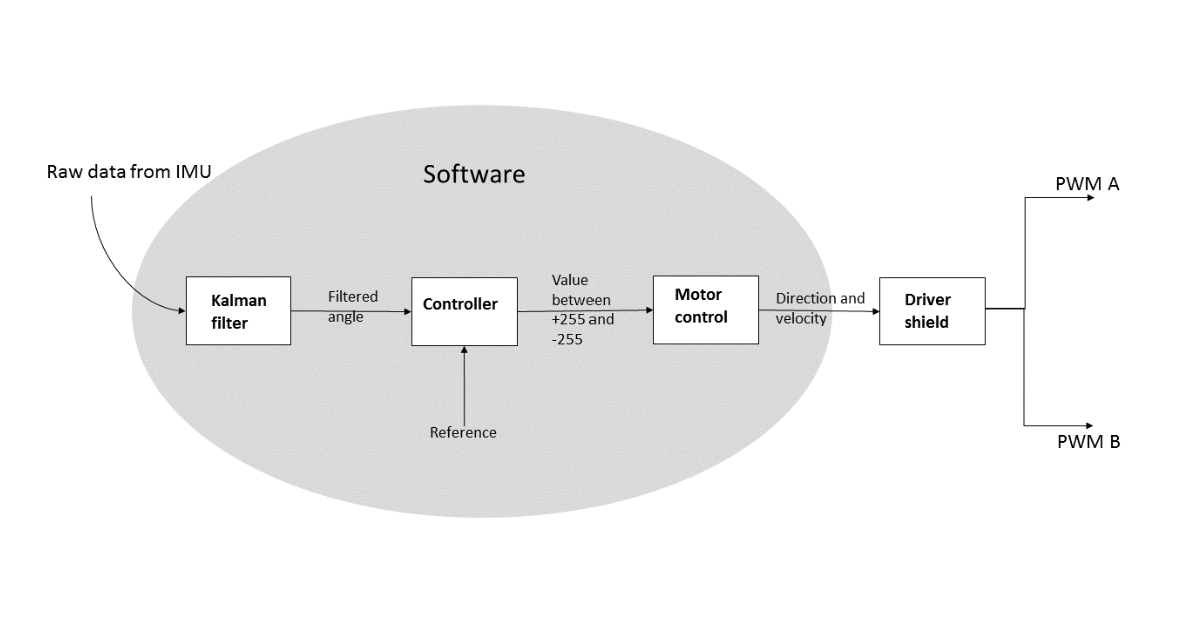
\includegraphics[height=8cm]{assets/pitch_angle_control_loop.png}
	\caption{A simplified diagram of the motor control loop \cite{10193276}.}
	\label{fig:schematics_control-loop}
\end{figure}


\subsubsection{Combined Results}
The use of PID controllers for pitch, yaw, and position control enables the robot to maintain balance and navigate effectively. The proportional, integral, and derivative terms in each PID loop allow the system to respond to real-time errors, minimize steady-state deviations, and anticipate future errors, leading to smooth and precise control of the robot's motion. The integration of these PID controllers is fundamental to the robot's stability and performance. The complete flow chart is shown in Fig.~\ref{fig:code-overview-flowchart} and the combined results are shown in Fig.~\ref{fig:final_pid}

\begin{figure}[h]
	\centering
	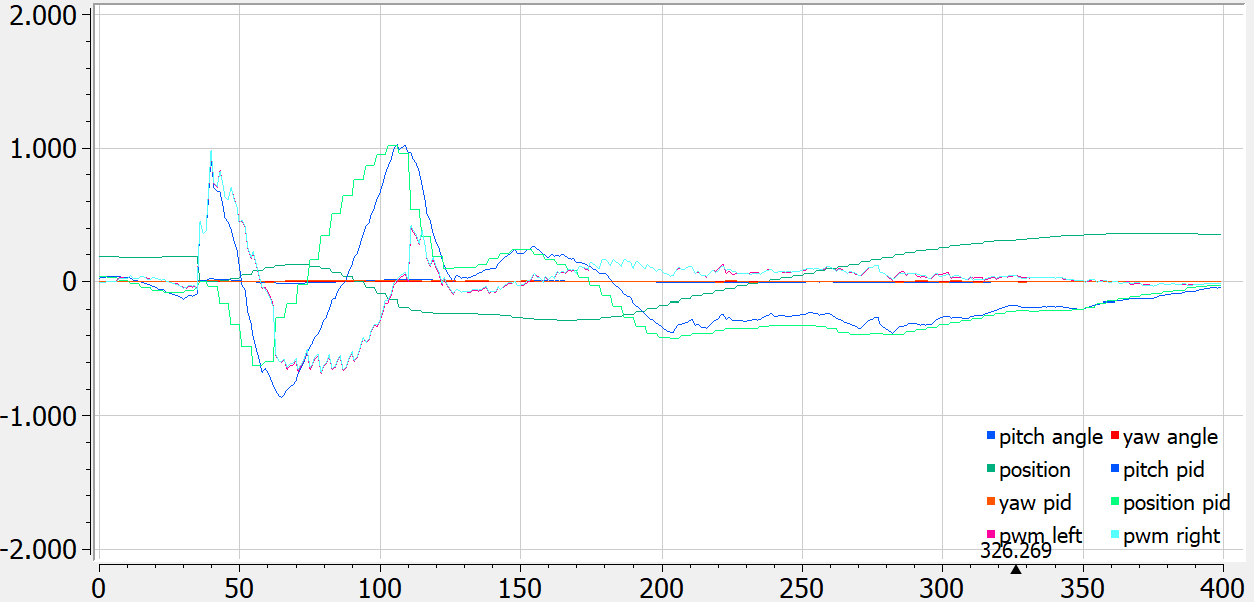
\includegraphics[width=0.8\linewidth]{assets/final_pid.png}
	\caption{The final control system individual output values recorded at baud rate of 115200.}
	\label{fig:final_pid}
\end{figure}


\begin{figure}[h]
	\centering
	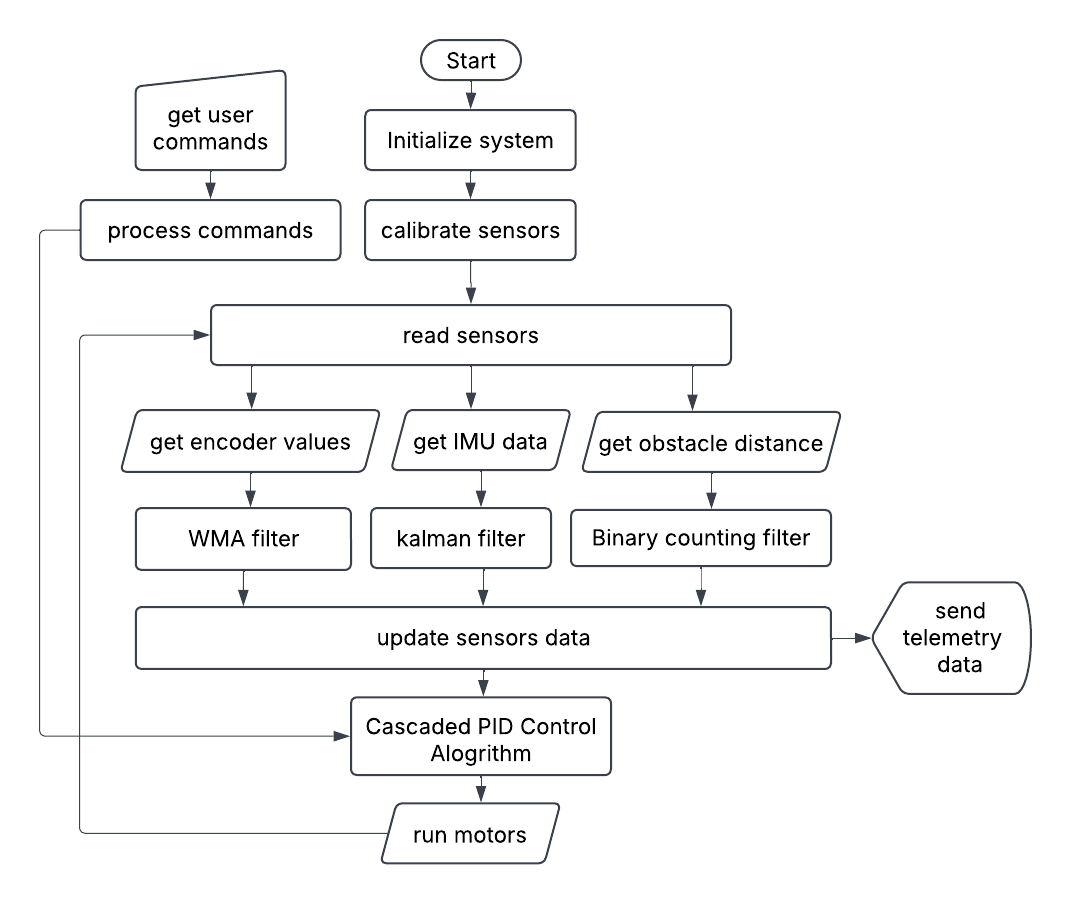
\includegraphics[width=0.8\linewidth]{assets/code_overview_flowchart.png}
	\caption{System operational flowchart for self-balancing mobile base.}
	\label{fig:code-overview-flowchart}
\end{figure}


\section{Front Obstacle Detection}
To robustly detect obstacles in its forward path, the robot employs a combination of an \textbf{ultrasonic distance-measuring sensor} and \textbf{infrared (IR) proximity sensors}. A simplified representation of the obstacle detection algorithm is depicted in Fig.~\ref{fig:obstacle_diagram}.

\begin{figure} [H]
	\centering
	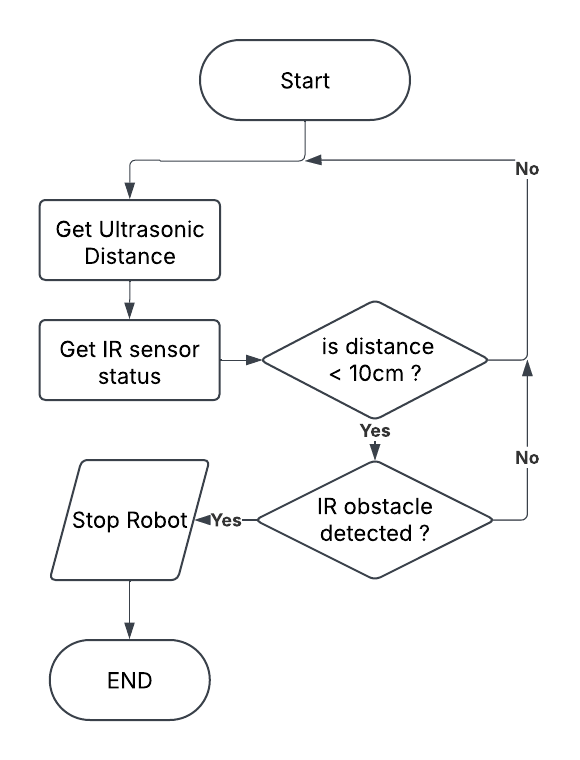
\includegraphics[height=9cm]{assets/obstacle_diagram}
	\caption{Flowchart for a robot's obstacle avoidance alogrithm using ultrasonic and infrared sensors.}
	\label{fig:obstacle_diagram}
\end{figure}


\subsubsection{Ultrasonic Distance Sensor} \label{HC-SR04}
The HC-SR04 is an ultrasonic distance sensor used for measuring the distance to an obstacle by sending an ultrasonic pulse and measuring the time it takes for the echo to return. It operates based on the principle of time-of-flight of sound waves, with a known speed of sound in air.
\begin{figure}[H]
	\centering
	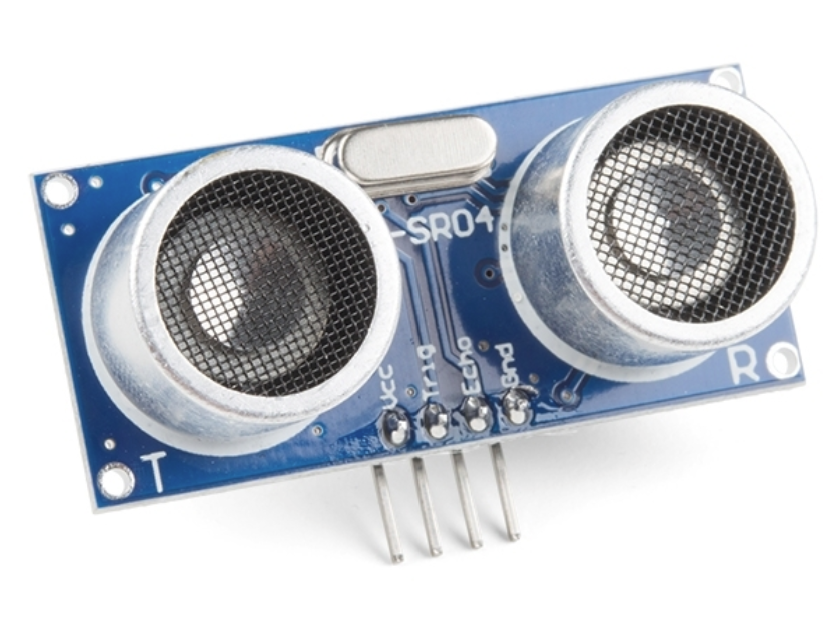
\includegraphics[width=0.25\linewidth]{assets/Ultrasonic-HC-SR04.png}
	\caption{Ultrasonic distance sensor by  Sparkfun electronics \cite{ultrasonic_sensor}.}
	\label{fig:ultra-sonic}
\end{figure}

\subsubsection{Infrared Sensing}  \label{IR_Intro}
The robot is equipped with infrared proximity sensors at the front-left and front-right directions using the Everlight Elec IR Receiver (IRM-56384) and the Infrared LED (IR204C-A). These sensors detect obstacles by transmitting a modulated infrared signal and detecting its reflection.
\begin{figure}[h]
	\centering
	\subfloat[IR204C-A \cite{ir_led}.]{
		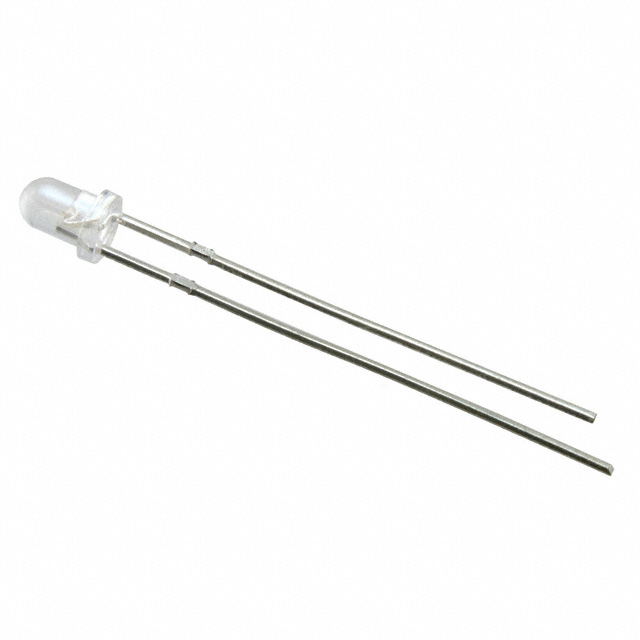
\includegraphics[height=4cm]{assets/HIR204C.jpg}
		\label{fig:ir-led}
	}
	\qquad
	\subfloat[IRM-56384 \cite{ir_receiver}.]{
		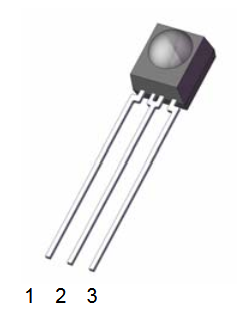
\includegraphics[height=4cm]{assets/ir-receiver.png}
		\label{fig:ir-receiver}
	}
	\caption{}
	\label{fig:ir-sensors}
\end{figure}

\subsection{Ultrasonic Working Principle}
As discussed in Section~\ref{HC-SR04}, the ultrasonic sensor operates based on the \textbf{time-of-flight} principle, utilizing sound waves to determine the distance to an obstacle. The sensor comprises two key components:
\begin{itemize}
	\item A \textbf{transmitter} that emits high-frequency ultrasonic pulses (typically at 40 kHz).
	\item A \textbf{receiver} that detects the reflected pulses after they bounce off an obstacle.
\end{itemize}

The distance to the obstacle is calculated by measuring the time delay between the transmission of the ultrasonic pulse and its reception. The formula used to compute the distance is:
\begin{equation}
	d = \frac{t \times v}{2}
\end{equation}
where:
\begin{itemize}
	\item \(d\) is the measured distance to the obstacle (in meters),
	\item \(t\) is the time delay between transmission and reception (in microseconds),
	\item \(v\) is the speed of sound in air (approximately 343 m/s at room temperature, 20°C).
\end{itemize}

\subsubsection{Ultrasonic Implementation}
The HC-SR04 requires control signals to be sent from a microcontroller:
\begin{enumerate}
	\item A short \textbf{trigger pulse} (at least 10 µs) is sent to the \texttt{TRIG} pin.
	\item The sensor responds with a high signal on the \texttt{ECHO} pin, the duration of which corresponds to the distance.
	\item The duration of the \texttt{ECHO} signal is measured to determine the distance.
\end{enumerate}

\subsubsection{Code for Distance Measurement}
Based on the datasheet \cite{ultrasonic_sensor}, an operating frequency of 20 Hz (corresponding to a 50 ms interval) is selected for distance measurements. The speed of sound is taken as 340.29 m/s, leading to the following constants in the code:

\begin{lstlisting}[style=cppstyle2]
constexpr uint8_t USONIC_GET_DISTANCE_DELAY_MS = 50; // Measurement interval
constexpr float SPEED_OF_SOUND_HALVED = (340.29 * 100.0) / (2 * 1000 * 1000); // Speed of sound in cm/us, divided by 2
\end{lstlisting}

\textbf{Code Explanation}:
\begin{itemize}
\item \texttt{USONIC\_GET\_DISTANCE\_DELAY\_MS}: Ensures measurements are taken at 20 Hz intervals.
\item \texttt{SPEED\_OF\_SOUND\_HALVED}: Converts the speed of sound to cm/µs and accounts for the round-trip travel time of the ultrasonic pulse.
\end{itemize}

The following C++ function initiates distance measurement using the HC-SR04 ultrasonic sensor:
\begin{lstlisting}[style=cppstyle2]
void StartUltrasonicMeasurement() {
	if (millis() - usonicGetDistancePrevTime > USONIC_GET_DISTANCE_DELAY_MS) {
		usonicMeasureFlag = SEND;
		usonicGetDistancePrevTime = millis(); // Update timestamp
		
		attachPinChangeInterrupt(ECHO_PIN, HandleUltrasonicMeasurementInterrupt, RISING); // Attach interrupt for rising edge
		
		digitalWrite(TRIG_PIN, LOW); 	// Reset TRIG pin
		delayMicroseconds(2);
		digitalWrite(TRIG_PIN, HIGH); 	// Send 10 us trigger pulse
		delayMicroseconds(10);
		digitalWrite(TRIG_PIN, LOW); 	// Reset TRIG pin
	}
}
\end{lstlisting}
\textbf{Code Explanation}:
\begin{itemize}
	\item The function \texttt{StartUltrasonicMeasurement()} ensures that the measurement is taken at regular intervals.
	\item A global flag \texttt{usonicMeasureFlag} is set to \texttt{SEND}, indicating that the trigger pulse is sent.
	\item The function \texttt{attachPinChangeInterrupt()} attaches an interrupt to detect when the \texttt{ECHO} pin goes HIGH.
	\item The \texttt{TRIG} pin is first set LOW (to reset), then HIGH (to trigger the pulse), and then set LOW again.
\end{itemize}
This setup enables precise distance measurement by capturing the time delay between sending and receiving the ultrasonic pulse.


\subsubsection{Interrupt Service Routine}
The following function handles the interrupt to measure the distance using the ultrasonic sensor:

\begin{lstlisting}[style=cppstyle2]
void HandleUltrasonicMeasurementInterrupt() {
	if (usonicMeasureFlag == SEND) {
		usonicMeasurePrevTime = micros();	// Record timestamp of rising edge
		attachPinChangeInterrupt(ECHO_PIN, HandleUltrasonicMeasurementInterrupt, FALLING);
		usonicMeasureFlag = RECEIVED; 	// Update flag to indicate echo reception
	} else if (usonicMeasureFlag == RECEIVED) {
		usonicDistanceValue = (uint8_t)((micros() - usonicMeasurePrevTime) * SPEED_OF_SOUND_HALVED);	// Compute distance
		usonicMeasureFlag = IDLE;	// Reset flag for next measurement
	}
}
\end{lstlisting}

\textbf{Code Explanation}:
\begin{enumerate}
	\item \textbf{Rising Edge Detection}:
	\begin{itemize}
		\item When the \texttt{ECHO} signal rises (RISING edge), the current time is recorded using \texttt{micros()}.
		\item The interrupt is reattached to detect the falling edge of the \texttt{ECHO} signal.
		\item The flag \texttt{usonicMeasureFlag} is updated to \texttt{RECEIVED} to indicate that the echo signal is being processed.
	\end{itemize}
	\item \textbf{Falling Edge Detection}:
	\begin{itemize}
		\item When the falling edge is detected, the elapsed time is computed as the difference between the current time and the previously recorded timestamp.		
		\item The distance is calculated using the formula:
		\begin{equation}
			d = \frac{ \Delta t \times v}{2}
		\end{equation}
		\item The flag \texttt{usonicMeasureFlag} is reset to \texttt{IDLE} to prepare for the next measurement cycle.
	\end{itemize}				
\end{enumerate}

\begin{itemize}
	\item When the \texttt{ECHO} signal rises (RISING edge), the timestamp is recorded using \texttt{micros()}.
	\item The interrupt is reattached to detect the falling edge of the \texttt{ECHO} signal.
	\item When the falling edge is detected, the elapsed time is computed and converted to distance using the speed of sound formula.
	\item The system resets for the next measurement by setting \texttt{usonicMeasureFlag} to \texttt{IDLE}.
\end{itemize}


\subsection{Infrared Sensing Implementation}
As discussed in Section~\ref{IR_Intro}, Infrared LED and Reciever.
The following code implements the control and processing logic for the \textbf{IR proximity sensors}:
\begin{lstlisting}[style=cppstyle2]
void IRSesorSend38KPule(unsigned char ir_pin){
	for( int i = 0; i < 39; i++) {
		digitalWrite(ir_pin, LOW);
		delayMicroseconds(9);
		digitalWrite(ir_pin, HIGH);
		delayMicroseconds(9);
	}
}

void ProcessLeftIRSensor(){
	if (millis() - irLeftCountTime > IR_COUNT_DELAY_MS) {
		UpdateSlidingWindow(irLeftPulseCount >= 3, irLeftHistory, irLeftIndex, irLeftRunningCount);    
		irLeftIsObstacle = (irLeftRunningCount >= 5); // Check if obstacle is detected
		irLeftPulseCount = 0;
		irLeftCountTime = millis(); // Update timestamp
	}
}

void ProcessRightIRSensor(){
	if (millis() - irRightCountTime > IR_COUNT_DELAY_MS) {
		UpdateSlidingWindow((irRightPulseCount >= 3), irRightHistory, irRightIndex, irRightRunningCount);
		irRightIsObstacle = (irRightRunningCount >= 5); // Check if obstacle is detected
		irRightPulseCount = 0; // Reset pulse coun
		irRightCountTime = millis(); // Update timestamp
	}
}
\end{lstlisting}

\textbf{Code Explanation}:
\begin{enumerate}
	\item \textbf{IR Pulse Generation}:
	\begin{itemize}
		\item The function \texttt{IRSensorSend38KPulse()} generates a 38 kHz modulated signal by toggling the IR LED pin at a specific frequency.
		\item Each cycle consists of 9 µs LOW and 9 µs HIGH states, repeated 39 times to ensure reliable signal transmission.
	\end{itemize}
	\item \textbf{Sensor Data Processing}:
	\begin{itemize}
		\item The functions \texttt{ProcessLeftIRSensor()} and \texttt{ProcessRightIRSensor()} process the data from the left and right IR sensors, respectively.
		\item A sliding window algorithm is used to filter out noise and improve detection reliability:
		\item The function \texttt{UpdateSlidingWindow()} updates a history buffer and running count of detected pulses. 
		\item An obstacle is considered detected if the running count exceeds a threshold (e.g., 5 out of 10 readings).
	\end{itemize}
	\item  \textbf{Obstacle Detection}:
	\begin{itemize}
		\item The flags \texttt{irLeftIsObstacle} and \texttt{irRightIsObstacle} indicate whether an obstacle is detected on the left or right side, respectively.		
		\item The pulse counts and timestamps are reset after each processing cycle to prepare for the next measurement.
	\end{itemize}
\end{enumerate}
\section{Remote Control and Communication}

The remote control and communication system of the two-wheeled self-balancing robot was designed to enable seamless and reliable interaction between the user and the robot. For this purpose, we integrated the BT16 Bluetooth UART Module, which provided a robust wireless communication link.

\subsection{Bluetooth Module Integration}
The BT16 Bluetooth UART Module is a high-performance component based on the Airoha ABI 602 chipset, compliant with the Bluetooth 4.2 BLE standard. It interfaces with the microcontroller via UART, ensuring efficient bidirectional data transmission. The module supports GATT-based communication through an integrated transparent data transmission service, enabling seamless and reliable Bluetooth connectivity.

A key feature of the BT16 module is its \textit{serial command mode}, which allows direct configuration and control via UART commands. Users can modify essential parameters, such as the UUID, device name, and connection settings, facilitating flexible integration into various applications.


\begin{figure}[H]
	\centering
	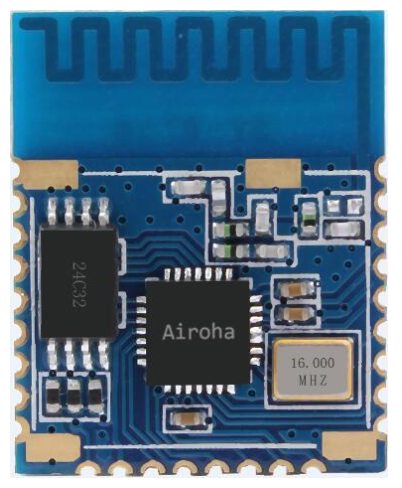
\includegraphics[height=3cm]{assets/BT16Module.png}
	\caption{Ultrasonic distance sensor by  Sparkfun electronics \cite{bluetooth_module}.}
	\label{fig:bluetooth}
\end{figure}



\subsection{Custom Communication Protocol}
A custom communication protocol was developed to manage the exchange of control commands and telemetry data, which is structured around well-defined command and telemetry packets, implemented in \texttt{comm.hpp}. These packets support multiple data formats, ensuring compatibility with various communication protocols. The functions responsible for sending and receiving telemetry data are listed in Tables~\ref{tab:uart_methods} and~\ref{tab:i2c_methods}.


\subsection{User Interfaces}
The user interface (UI) for the robot is designed to facilitate interactive control and real-time monitoring. It integrates command parsing, telemetry data handling, and communication protocols such as Inter-Integrated Circuit (I2C) and Universal Asynchronous Receiver-Transmitter (UART). Users can send commands to the robot and receive real-time telemetry feedback, ensuring efficient control and monitoring.

\subsection{UART Communication}
The Universal Asynchronous Receiver-Transmitter (UART) protocol is used for serial communication, typically with a Bluetooth module or a computer for debugging and remote control. The communication is initialized at a baud rate of \texttt{9600}, which is commonly used for Bluetooth modules \cite{bluetooth_module}.

\begin{table}[h]
	\centering
	\caption{UART Communication Methods}
	\begin{tabular}{|l|l|l|}
		\hline
		\textbf{Packet Type} & \textbf{Function} & \textbf{Description} \\ \hline
		\multirow{4}{*}{Command Packets} & \texttt{readUartBytes()} & Reads command data as raw bytes. \\ \cline{2-3}
		& \texttt{readUartASCII()} & Reads command data as an ASCII string. \\ \cline{2-3}
		& \texttt{sendUartBytes()} & Sends command data as raw bytes. \\ \cline{2-3}
		& \texttt{sendUartASCII()} & Sends command data as an ASCII string. \\ \hline
		\multirow{4}{*}{Telemetry Packets} & \texttt{sendUartBytes()} & Sends telemetry data as raw bytes. \\ \cline{2-3}
		& \texttt{sendUartASCII()} & Sends telemetry data as an ASCII string. \\ \cline{2-3}
		& \texttt{readUartBytes()} & Reads telemetry data as raw bytes. \\ \cline{2-3}
		& \texttt{readUartASCII()} & Reads telemetry data as an ASCII string. \\ \hline
	\end{tabular}
	\label{tab:uart_methods}
\end{table}

\subsection{I2C Communication}
Inter-Integrated Circuit (I2C) communication is used for short-range, two-wire serial communication. The robot operates as an I2C slave with a predefined address (SLAVE\_ADDR = 8), allowing it to receive commands and transmit telemetry data over the I2C bus.

\begin{table}[h]
	\centering
	\caption{I2C Communication Methods}
	\begin{tabular}{|l|l|l|}
		\hline
		\textbf{Packet Type} & \textbf{Function} & \textbf{Description} \\ \hline
		\multirow{4}{*}{Command Packets} & \texttt{sendI2CBytes(addr)} & Sends command data as raw bytes to the address. \\ \cline{2-3}
		& \texttt{sendI2CASCII(addr)} & Sends command data as ASCII to the address. \\ \cline{2-3}
		& \texttt{readI2CBytes(addr)} & Reads command data as raw bytes from the address. \\ \cline{2-3}
		& \texttt{readI2CASCII(addr)} & Reads command data as ASCII from the address. \\ \hline
		\multirow{4}{*}{Telemetry Packets} & \texttt{sendI2CBytes()} & Sends telemetry data as raw bytes. \\ \cline{2-3}
		& \texttt{sendI2CASCII()} & Sends telemetry data as ASCII. \\ \cline{2-3}
		& \texttt{readI2CBytes(addr)} & Reads telemetry data as raw bytes from the address. \\ \cline{2-3}
		& \texttt{readI2CASCII(addr)} & Reads telemetry data as ASCII from the address. \\ \hline
	\end{tabular}
	\label{tab:i2c_methods}
\end{table}

\subsection{Sending Commands}
Users can send commands to control the robot’s movement, rotation, or stop function. Commands follow a predefined structured format and can be transmitted via either I2C or UART. The available commands are listed in Table~\ref{tab:commands}.

\textbf{ASCII Format}:
The commands sent in ASCII is formatted as a comma-separated string:
\begin{lstlisting}[]
	<command>,<command_value>,<command_speed>
\end{lstlisting}

\begin{table}[H]
	\centering
	\caption{List of Commands and Corresponding Values}
	\label{tab:commands}
	\begin{tabular}{|c|c|l|}
		\hline
		\textbf{Command} & \textbf{Value} & \textbf{Description} \\ \hline
		\texttt{Stop}     & 0              & Stops the robot's movement. \\ \hline
		\texttt{Move}     & 1              & Moves forward or backward (in cm) at a given speed. \\ \hline
		\texttt{Rotate}   & 2              & Rotates the robot by a angle (in degrees) at a given speed. \\ \hline
		\texttt{INVALID}  & 3              & Represents an invalid or unrecognized command. \\ \hline
	\end{tabular}
\end{table}

\textbf{Example Command:}
\begin{itemize}
	\item Stop the robot: \texttt{0}
	\item Move forward 100 cm at 50\% speed:  \texttt{1,100,50}
	\item Rotate 90° at 30 speed\%: \texttt{2,90,30}
\end{itemize}

\subsection{Receiving Telemetry Data}
The robot continuously monitors its state and environment using onboard sensors. This data is packaged into a structured format and transmitted back to the user for real-time monitoring and feedback. Telemetry data includes:
\begin{itemize}
	\item \textbf{Yaw Angle}: The robot's current orientation in degrees.
	\item \textbf{Distance Traveled}: The total distance traveled by the robot in centimeters.
	\item \textbf{Ultrasonic Distance}: The distance to the nearest obstacle, as measured by the ultrasonic sensor in centimeters.
\end{itemize}

\textbf{ASCII Format}:
The telemetry data recieved in ASCII is formatted as a comma-separated string:
\begin{lstlisting}[]
	<yaw_angle>,<distance_traveled>,<ultrasonic_distance>
\end{lstlisting}
\textbf{Example Output}:
\begin{lstlisting}[]
	45,200,30
\end{lstlisting}

This indicates a yaw angle of 45 degrees, a distance traveled of 200 cm, and an ultrasonic reading of 30 cm.


%\section{Simulation and Testing}
Simulation and testing played a crucial role in the development and refinement of the two-wheeled self-balancing robot. By leveraging computational tools and environments, we were able to model the robot's behavior under various conditions, validate control algorithms, and predict system performance before real-world implementation.

\subsection{Simulation Tools and Environment}
For simulating the dynamics and control strategies of the robot, we utilized both \textbf{Python} and \textbf{MATLAB}. These platforms provided robust frameworks for numerical computation, visualization, and algorithm development.

\begin{itemize}
\item \textbf{Python:} Utilized libraries such as \textit{NumPy}, \textit{SciPy}, and \textit{Matplotlib} for numerical simulations and visualizations. \textit{Control} and \textit{SymPy} libraries were used to model the control systems and analyze the system's response.
\item \textbf{MATLAB:} Employed for more advanced control design and simulation, including the use of Simulink for block diagram modeling and simulation of dynamic systems. MATLAB's built-in tools facilitated the tuning and optimization of control parameters.
\end{itemize}

\subsection{Control Algorithm Testing}
We implemented and tested various control algorithms to ensure the stability and performance of the robot. Key focus was given to the \textbf{Complementary Filter} and \textbf{Kalman Filter} for sensor fusion and state estimation.

\begin{itemize}
\item \textbf{Complementary Filter:} Simulations helped fine-tune the filter coefficients to effectively merge accelerometer and gyroscope data, providing a stable estimate of the robot's tilt angle.
\item \textbf{Kalman Filter:} The filter was tested for its ability to reduce noise and provide accurate state estimation. MATLAB simulations were crucial in visualizing the filter's performance and adjusting the covariance matrices.
\end{itemize}

\subsection{Performance Metrics}
Several metrics were used to evaluate the performance of the control algorithms in the simulation environment:

\begin{itemize}
\item \textbf{Stability:} Assessed by analyzing the system's ability to return to an upright position after disturbances.
\item \textbf{Response Time:} Measured how quickly the control system could react to changes in tilt and external perturbations.
\item \textbf{Noise Rejection:} Evaluated the effectiveness of the filters in minimizing sensor noise and maintaining accurate state estimation.
\end{itemize}

\subsection{Real-World Validation}
Post-simulation, the control algorithms were transferred to the physical robot for real-world testing. The outcomes from the simulations provided a strong baseline, and discrepancies observed during physical trials were fed back into the simulation models for further refinement. This iterative process ensured a robust and reliable control system.

Overall, the combination of Python and MATLAB simulations significantly accelerated the development process and provided valuable insights into the robot's dynamic behavior and control performance.

\section{Simulation and Testing}

Simulation and testing played a crucial role in the development and refinement of the two-wheeled self-balancing robot. By leveraging computational tools and environments, we were able to model the robot's behavior under various conditions, validate control algorithms, and predict system performance before real-world implementation.

\subsection{Simulation Tools and Environment}
For simulating the dynamics and control strategies of the robot, we utilized both \textbf{Python} and \textbf{MATLAB}. These platforms provided robust frameworks for numerical computation, visualization, and algorithm development.

\subsection{PID Tuning}
\subsubsection{}
\subsubsection{PID Tuning Results}
Response specifications No Load With Loads 
Initial Deviation 
Rise Time
Peak Time
Maximum Overshoot
Settling Time
Error Steady State

\begin{itemize}
\item \textbf{Python:} Utilized libraries such as \textit{NumPy}, \textit{SciPy}, and \textit{Matplotlib} for numerical simulations and visualizations. \textit{Control} and \textit{SymPy} libraries were used to model the control systems and analyze the system's response.
\item \textbf{MATLAB:} Employed for more advanced control design and simulation, including the use of Simulink for block diagram modeling and simulation of dynamic systems. MATLAB's built-in tools facilitated the tuning and optimization of control parameters.
\end{itemize}

\subsection{Control Algorithm Testing}
We implemented and tested various control algorithms to ensure the stability and performance of the robot. Key focus was given to the \textbf{Complementary Filter} and \textbf{Kalman Filter} for sensor fusion and state estimation.

\begin{itemize}
\item \textbf{Complementary Filter:} Simulations helped fine-tune the filter coefficients to effectively merge accelerometer and gyroscope data, providing a stable estimate of the robot's tilt angle.
\item \textbf{Kalman Filter:} The filter was tested for its ability to reduce noise and provide accurate state estimation. MATLAB simulations were crucial in visualizing the filter's performance and adjusting the covariance matrices.
\end{itemize}

\subsection{Performance Metrics}
Several metrics were used to evaluate the performance of the control algorithms in the simulation environment:

\begin{itemize}
\item \textbf{Stability:} Assessed by analyzing the system's ability to return to an upright position after disturbances.
\item \textbf{Response Time:} Measured how quickly the control system could react to changes in tilt and external perturbations.
\item \textbf{Noise Rejection:} Evaluated the effectiveness of the filters in minimizing sensor noise and maintaining accurate state estimation.
\end{itemize}

\subsection{Real-World Validation}
Post-simulation, the control algorithms were transferred to the physical robot for real-world testing. The outcomes from the simulations provided a strong baseline, and discrepancies observed during physical trials were fed back into the simulation models for further refinement. This iterative process ensured a robust and reliable control system.


To thoroughly test the robustness of the system, we introduced controlled disturbances and varying surface conditions in the real-world environment. This helped identify edge cases and stress points that were not evident in the simulation phase. By iteratively refining the control algorithms based on these findings, we were able to enhance the overall stability and performance of the robot.

Overall, the combination of Python and MATLAB simulations significantly accelerated the development process and provided valuable insights into the robot's dynamic behavior and control performance.


%\section{Power Management}

Efficient power management was critical for ensuring the longevity and reliability of the two-wheeled self-balancing robot. We employed \textbf{7.4V Lithium-Ion battery packs} to provide a stable power supply.

\subsection{Battery Selection and Integration}
The 7.4V Lithium-Ion battery packs were chosen for their high energy density, lightweight properties, and reliable performance. These batteries were integrated with a voltage regulator circuit to ensure consistent voltage levels to the microcontroller and motor drivers.

\subsection{Power Monitoring}
To monitor the battery status in real-time, voltage sensors were used to track battery levels. This data was integrated into the telemetry feedback system, allowing the user to receive alerts when the battery level was low.

\subsection{Charging and Safety}
A dedicated charging circuit with overcharge protection was implemented to enhance battery life and safety. Thermal sensors were also included to monitor battery temperature during operation and charging.
\section{User Interface}
The user interface (UI) for the robot is designed to facilitate interactive control and real-time monitoring. It integrates command parsing, telemetry data handling, and communication protocols such as Inter-Integrated Circuit (I2C) and Universal Asynchronous Receiver-Transmitter (UART). Users can send commands to the robot and receive real-time telemetry feedback, ensuring efficient control and monitoring.

Communication is structured around well-defined command and telemetry packets, implemented in \texttt{comm.hpp}. These packets support multiple data formats, ensuring compatibility with various communication protocols. The functions responsible for sending and receiving telemetry data are listed in Tables~\ref{tab:uart_methods} and~\ref{tab:i2c_methods}.

\subsection{UART Communication}
The Universal Asynchronous Receiver-Transmitter (UART) protocol is used for serial communication, typically with a Bluetooth module or a computer for debugging and remote control. The communication is initialized at a baud rate of \texttt{9600}, which is commonly used for Bluetooth modules \cite{bluetooth}.

\begin{table}[h]
	\centering
	\caption{UART Communication Methods}
	\begin{tabular}{|l|l|l|}
		\hline
		\textbf{Packet Type} & \textbf{Function} & \textbf{Description} \\ \hline
		\multirow{4}{*}{Command Packets} & \texttt{readUartBytes()} & Reads command data as raw bytes. \\ \cline{2-3}
		& \texttt{readUartASCII()} & Reads command data as an ASCII string. \\ \cline{2-3}
		& \texttt{sendUartBytes()} & Sends command data as raw bytes. \\ \cline{2-3}
		& \texttt{sendUartASCII()} & Sends command data as an ASCII string. \\ \hline
		\multirow{4}{*}{Telemetry Packets} & \texttt{sendUartBytes()} & Sends telemetry data as raw bytes. \\ \cline{2-3}
		& \texttt{sendUartASCII()} & Sends telemetry data as an ASCII string. \\ \cline{2-3}
		& \texttt{readUartBytes()} & Reads telemetry data as raw bytes. \\ \cline{2-3}
		& \texttt{readUartASCII()} & Reads telemetry data as an ASCII string. \\ \hline
	\end{tabular}
	\label{tab:uart_methods}
\end{table}

\subsection{I2C Communication}
Inter-Integrated Circuit (I2C) communication is used for short-range, two-wire serial communication. The robot operates as an I2C slave with a predefined address (SLAVE\_ADDR = 8), allowing it to receive commands and transmit telemetry data over the I2C bus.

\begin{table}[h]
	\centering
	\caption{I2C Communication Methods}
	\begin{tabular}{|l|l|l|}
		\hline
		\textbf{Packet Type} & \textbf{Function} & \textbf{Description} \\ \hline
		\multirow{4}{*}{Command Packets} & \texttt{sendI2CBytes(addr)} & Sends command data as raw bytes to the specified address. \\ \cline{2-3}
		& \texttt{sendI2CASCII(addr)} & Sends command data as ASCII to the specified address. \\ \cline{2-3}
		& \texttt{readI2CBytes(addr)} & Reads command data as raw bytes from the specified address. \\ \cline{2-3}
		& \texttt{readI2CASCII(addr)} & Reads command data as ASCII from the specified address. \\ \hline
		\multirow{4}{*}{Telemetry Packets} & \texttt{sendI2CBytes()} & Sends telemetry data as raw bytes. \\ \cline{2-3}
		& \texttt{sendI2CASCII()} & Sends telemetry data as ASCII. \\ \cline{2-3}
		& \texttt{readI2CBytes(addr)} & Reads telemetry data as raw bytes from the specified address. \\ \cline{2-3}
		& \texttt{readI2CASCII(addr)} & Reads telemetry data as ASCII from the specified address. \\ \hline
	\end{tabular}
	\label{tab:i2c_methods}
\end{table}

\subsection{Sending Commands}
Users can send commands to control the robot’s movement, rotation, or stop function. Commands follow a predefined structured format and can be transmitted via either I2C or UART. The available commands are listed in Table~\ref{tab:commands}.

\textbf{ASCII Format}:
The commands sent in ASCII is formatted as a comma-separated string:
\begin{lstlisting}[]
	<command>,<command_value>,<command_speed>
\end{lstlisting}

\begin{table}[H]
	\centering
	\caption{List of Commands and Corresponding Values}
	\label{tab:commands}
	\begin{tabular}{|c|c|l|}
		\hline
		\textbf{Command} & \textbf{Value} & \textbf{Description} \\ \hline
		\texttt{Stop}     & 0              & Stops the robot's movement. \\ \hline
		\texttt{Move}     & 1              & Moves forward or backward (in cm) at a given speed. \\ \hline
		\texttt{Rotate}   & 2              & Rotates the robot by a specified angle (in degrees) at a given speed. \\ \hline
		\texttt{INVALID}  & 3              & Represents an invalid or unrecognized command. \\ \hline
	\end{tabular}
\end{table}

\textbf{Example Command:}
\begin{itemize}
	\item Stop the robot: \texttt{0}
	\item Move forward 100 cm at 50\% speed:  \texttt{1,100,50}
	\item Rotate 90° at 30 speed\%: \texttt{2,90,30}
\end{itemize}

\subsection{Receiving Telemetry Data}
The robot continuously monitors its state and environment using onboard sensors. This data is packaged into a structured format and transmitted back to the user for real-time monitoring and feedback. Telemetry data includes:
\begin{itemize}
	\item \textbf{Yaw Angle}: The robot's current orientation in degrees.
 	\item \textbf{Distance Traveled}: The total distance traveled by the robot in centimeters.
	\item \textbf{Ultrasonic Distance}: The distance to the nearest obstacle, as measured by the ultrasonic sensor in centimeters.
\end{itemize}

\textbf{ASCII Format}:
The telemetry data recieved in ASCII is formatted as a comma-separated string:
\begin{lstlisting}[]
	<yaw_angle>,<distance_traveled>,<ultrasonic_distance>
\end{lstlisting}
\textbf{Example Output}:
\begin{lstlisting}[]
	45,200,30
\end{lstlisting}

This indicates a yaw angle of 45 degrees, a distance traveled of 200 cm, and an ultrasonic reading of 30 cm.

\section{Safety Features}
Ensuring the safety of both the robot and its environment was a priority in the design process. Multiple safety features were integrated into the system.

\subsection{Emergency Stop Mechanism}
A robust emergency stop system allows the robot to be immediately powered down in critical situations. This can be triggered either by a physical emergency stop button or remotely via a wireless command. This feature ensures quick intervention in the event of a malfunction or hazardous condition.

\subsection{Overcurrent and Overvoltage Protection}
To prevent electrical damage, the system incorporates dedicated protection circuits that monitor current and voltage levels in real time. If an overcurrent or overvoltage condition is detected, power is automatically cut off to safeguard the motors and microcontroller, preventing potential failures or overheating.

\subsection{Fall Detection and Recovery}
The robot is equipped with sensors that continuously monitor its tilt angle. If the robot tips beyond a predefined threshold, indicating a potential fall, the motors are automatically disabled to prevent further damage. Additionally, a self-recovery sequence can be initiated, allowing the robot to regain an upright position without human intervention.
\section{Future Work and Improvements}
While the current implementation of the two-wheeled self-balancing robot demonstrates robust performance, several areas can be further improved to enhance functionality, autonomy, and user experience.


\subsection{Advanced Control Strategies}
Implementing more sophisticated control algorithms, such as adaptive controllers or reinforcement learning-based approaches, could improve stability and dynamic response under varying conditions. Model predictive control (MPC) could also be explored to optimize real-time decision-making.


\subsection{Autonomous Navigation and Perception}
Enhancing the robot’s autonomy by integrating additional sensors such as LiDAR or depth cameras would enable precise environmental perception. Implementing SLAM (Simultaneous Localization and Mapping) algorithms would allow the robot to navigate and map complex environments independently.


\subsection{Seamless Mobile Integration}
Developing a dedicated mobile application with an intuitive user interface and real-time data visualization could significantly improve remote operation. Features such as wireless control, customizable movement presets, and telemetry monitoring would enhance usability.

\subsection{Optimized Power Management}
Exploring high-efficiency battery technologies, regenerative braking mechanisms, and smart power management systems could extend the robot’s operational lifespan. Additionally, integrating energy-efficient motor drivers and optimizing power consumption could further enhance performance.

By addressing these areas, the robot’s capabilities could be significantly expanded, paving the way for more advanced applications in research, automation, and real-world deployment.y management systems could extend the robot's operational time.
%\include{real_world_applications.tex}
%\section{Challenges and Limitations}

Throughout the development process, several challenges and limitations were encountered.

\subsection{Sensor Noise and Drift}
Despite the use of Kalman and Complementary filters, sensor noise and drift remained a challenge, affecting the accuracy of state estimation.

\subsection{Hardware Constraints}
Limitations in processing power and memory on the microcontrollers constrained the complexity of algorithms that could be implemented.

\subsection{Battery Life}
While the 7.4V Lithium-Ion battery packs provided adequate power, extended operation times required frequent recharging, highlighting the need for more efficient power management.

\subsection{Communication Interference}
Bluetooth communication was susceptible to interference in noisy environments, occasionally affecting the reliability of remote control.

Addressing these challenges will be key in future iterations to enhance the robustness and functionality of the system.



\bibliographystyle{IEEEtran}
\bibliography{references.bib}

\end{document}